\documentclass[a4paper,oneside]{book}


% Интерфейсы
\usepackage{Labnik}
% Заплатка для отрисовка архичных рисунков и прочих атавизмов
\usepackage{Labnik-III-patch}

\begin{document}

\chapter{Носители электрического тока}
\todo[author=Nozik, inline]{Название главы?}

Электрический ток представляет собой направленный перенос зарядов. Микрочастицы,
осуществляющие этот перенос, называют \term{носителями тока}. В~простейшем
случае носителями тока являются заряженные частицы,
движущиеся в свободном от вещества пространстве (ток в вакуумном диоде,
ионный пучок в масс-спектрометре, и т.\,д.).
Как правило, это электроны~--- элементарные частицы с известными значениями заряда
$q_e=-e\approx-1,6\cdot 10^{-19}\;Кл$
и массы
$m_e\approx 9,1\cdot 10^{-31}\;кг$.

Понятие \term{носители тока в веществе} уже не является таким наглядным.
Хотя в металлах и полупроводниках перенос заряда происходит
вследствие перемещения всё тех же электронов, их движение уже не является
движением свободных частиц, как в вакууме. Электроны движутся в сильном
периодическом поле, образованном ионами кристаллической решётки, и
взаимодействуют между собой, причём это движение и это взаимодействие
подчиняются законам квантовой механики. По этим законам получается, что такое
движение можно по-прежнему интерпретировать как движение свободных заряженных
частиц, но масса этих частиц, называемая \term{эффективной массой},
\important{не совпадает с массой свободного электрона},
$m_{e}^{эфф}\ne m_e$.
Более того, полупроводники и некоторые металлы ведут себя так,
будто вместо электронов ток в них переносят некоторые положительные частицы~---
так называемые \term{дырки}. Дырки подобны элементарным
частицам позитронам~--- в электрических и магнитных полях они движутся
как положительно заряженные частицы с зарядом $q_p=+e$,
но с некоторой эффективной массой $m_p^{эфф}\ne m_e$.

Таким образом, в физике металлов и полупроводников в качестве носителей тока
рассматривают \term{квазичастицы},
\important{не существующие отдельно от рассматриваемого вещества}.
Заряд этих носителей численно точно равен заряду электрона и может быть как
отрицательным, так и положительным. В~первом случае они по-прежнему называются
\term{электронами} (хотя их масса не равна $m_e$),
во втором~--- \term{дырками}. В~полупроводниках присутствуют оба типа этих
носителей, в большинстве металлов имеются только отрицательные носители.

\todo[inline,author=Popov,color=cyan]{Интегрировать с текстом выше --->}
% \paragraph{Определение элементарного заряда.}
Первые точные измерения элементарного заряда были выполнены Робертом Милликеном
в классических опытах в 1908--1916 годов. Идея этих опытов достаточно проста.
Если элементарный заряд действительно существует, то величина заряда~$q$ любого
тела может принимать только дискретную последовательность значений:
\begin{equation*}
	q = 0,\,\pm e,\,\pm2e,\,\pm3e,\, \ldots
\end{equation*}
где $e$~--- элементарный заряд.

В~опыте Милликена измерялся электрический заряд капелек масла микроскопических
размеров, несущих всего несколько элементарных зарядов.
Сравнивая между собой заряды капель, можно убедиться в том, что все они кратны
одному и тому же числу~--- заряду электрона.
\todo[inline,color=cyan]{<---}

\todo[inline,author=Popov,color=cyan]{Перенести в описание работы --->}
Измерение заряда капель производится путём исследования их движения в
электрическом поле. В~расположенный горизонтально плоский конденсатор через
отверстие в верхней пластине впрыскиваются мелкие капельки масла, получаемые с
помощью специального распылителя. На пластины конденсатора подаётся постоянное
напряжение (порядка нескольких киловольт). В~ходе опыта это напряжение можно
изменять. При распылении капельки масла вследствие трения о воздух приобретают
случайный по величине и знаку электрический заряд. Попадая в конденсатор,
капельки масла движутся в воздухе, опускаясь под действием силы тяжести или
поднимаясь под действием электрического поля. Время~$t_0$ опускания капли и
время её обратного подъёма~$t$ легко измерить с необходимой точностью.
Оказывается, что именно к измерению этих двух интервалов времени и сводится
измерение заряда капли.

Разумеется, дискретность заряда разных капель и, следовательно, величина
элементарного заряда, то есть заряд электрона, могут быть обнаружены только в
том случае, если абсолютная ошибка в измерении заряда капли будет существенно
меньше самого элементарного заряда. В~опытах Милликена необходимая точность
вполне может быть обеспечена в условиях лабораторного практикума.
\todo[inline,color=cyan]{<---}


\introsection{Движение заряженных частиц в электрических и магнитных полях}

Рассмотрим несколько примеров движения электронов в вакууме под действием
электрического и магнитного полей. Такие условия движения реализуются,
например, в электронных вакуумных приборах, таких, как электронно-лучевая
трубка или вакуумный диод.

% Эти относительно несложные и наглядные примеры позволят нам понять, как можно
% измерить такую важную характеристику заряженной частицы, как отношение её
% заряда к её массе~$e/m$ (удельный заряд частицы).

\introsubsection{Движение заряда в однородном магнитном поле}

Как известно, на заряд~$q$, движущийся со скоростью~$\vec{v}$ в магнитном поле
$\vec{B}$, действует \term{сила Лоренца}:
\begin{equation*}
    \eqmark{3.1}
	\vec{F}=q{\vec{v}}\times{\vec{B}}.
\end{equation*}

Рассмотрим точечный заряд, движущийся с некоторой скоростью~$\vec{v}$
в однородном магнитном поле $\vec{B}=\const$, перпендикулярном направлению скорости,
$\vec{v}\bot \vec{B}$. На движущийся электрон действует сила
\begin{equation*}
	F=qvB.
\end{equation*}
Эта сила перпендикулярна скорости движения, и не изменяет поэтому
её абсолютной величины. Траектория движения заряда в этом случае является
\important{окружностью}. Такое движение частицы называется \term{циклотронным вращением}.

Вычислим радиус~$R$ этой окружности, называемый
\term{ларморовским радиусом}, и угловую скорость циклотронного
вращения~$\omega_c$~--- так называемую \term{циклотронную частоту}.
Сила~$F$ является центростремительной, поэтому
$m\frac{v^2}{R}=evB$, где $m=m_e$, откуда находим
\begin{equation}
	\eqmark{3.2}
    R =\frac{m v}{qB}= \frac{v}{\omega_c},
\end{equation}
где
\begin{equation*}
	\omega_c=\frac{eB}{m}
\end{equation*}
---~циклотронная частота электрона. Важно заметить, что циклотронная частота не
зависит от энергии частицы, так что в однородном магнитном поле все электроны,
находящиеся в рассматриваемом объёме, вращаются с одинаковой частотой.

Скорость движения электрона можно найти, зная разность потенциалов~$V$,
пройденную электроном:
\begin{equation*}
	\frac{mv^2}{2}=eV,
\end{equation*}
откуда
\begin{equation}
	\omega_c=\frac{qB}{m}.
\end{equation}
Заметим, что циклотронная частота не зависит от энергии частицы,
так что в однородном магнитном поле все частицы одного типа (например,
электроны) вращаются с \important{одинаковой} частотой.
Частицы с разными знаками заряда вращаются в разные стороны.

Пусть теперь заряд движется в магнитном поле под некоторым углом~$\alpha$ к
вектору индукции~$\vec{B}$. Скорость заряда~$\vec{v}$ можно разложить
на две составляющие: перпендикулярную и параллельную магнитному полю:
\begin{equation*}
	v_{\bot}=v\sin\alpha,\qquad v_{\parallel}=v\cos\alpha.
\end{equation*}

Параллельная составляющая скорости не вызывает появление силы Лоренца, поэтому
проекция траектории на плоскость, перпендикулярную~$\vec{B}$,
по-прежнему представляет собой окружность с ларморовским радиусом,
определяемым поперечной составляющей скорости:
\begin{equation}
	\eqmark{3.4}
	R =\frac{m v_{\bot}}{eB}.
\end{equation}
В~направлении поля~$\vec{B}$ на заряд не действуют никакие силы,
следовательно, в этом направлении он движется равномерно со скоростью
$v_{\parallel}$.
Траектория заряда представляет собой \important{винтовую линию}.

\todo[inline,author=Popov,color=cyan]{Убрать в описание работы --->}
\paragraph{Метод магнитной фокусировки для измерения $e/m$.}
Найдём расстояние~$L$, которое проходит электрон в направлении вдоль поля за один
оборот (шаг винтовой линии). Время одного оборота~$T_c$,
называемое \term{циклотронным периодом}, равно
$T_c= \frac{2\pi R}{v_{\bot}}$. Заменяя $R/v_{\bot}$ c помощью \eqref{3.4}, найдём
\begin{equation}
	\eqmark{3.5}
	T_c =\frac{2\pi m}{eB}.
\end{equation}

За это время электрон проходит вдоль магнитного поля расстояние
\begin{equation}
	\eqmark{3.6}
    L = v_{\parallel}T_c =\frac{2\pi v\cos\alpha}{(e/m)B}.
\end{equation}

Если углы невелики $\alpha \ll 1$, то $\cos\alpha \approx 1$ и
\begin{equation}
	\eqmark{3.7}
    L \approx \frac{2\pi v}{(e/m)B}.
\end{equation}
Таким образом, при малых углах расстояние~$L$ не зависит от~$\alpha$, так
что все электроны, вышедшие из одной точки, после одного оборота вновь соберутся
в одной точке~--- сфокусируются. Как следует из \eqref{3.7}, индукция поля~$B$,
при которой точка фокусировки отстоит от точки вылета на расстоянии~$L$, зависит
от величины~$e/m$~--- удельного заряда электрона.

Скорость движения электрона определяется разность потенциалов~$V$,
пройденную им до попадания в магнитное поле:
\begin{equation*}
  \frac{mv^2}{2}=eV,
\end{equation*}
откуда
\begin{equation}
  \eqmark{3.3}
  v=\sqrt{\frac{2eV}{m}}.
%   = 6\cdot10^5\sqrt{V}~\frac{m}{c}.
\end{equation}

Обозначим через~$B_ф$ индукцию магнитного поля, при которой наступает фокусировка.
Используя \eqref{3.3} и \eqref{3.7}, выразим удельный заряд электрона~$e/m$ через~$B_ф$:
\begin{equation}
\eqmark{3.8}
\frac{e}{m}=\frac{8\pi^2 V}{L^2B_ф^2}.
\end{equation}
Эта формула положена в основу экспериментального измерения удельного заряда
электрона по \important{методу магнитной фокусировки}.
\todo[inline,color=cyan]{<---}

\introsubsection{Движение электрона в скрещенных электрическом и магнитном полях}

\todo[inline,author=Popov,color=green]{Вставить этот текст -->}
Рассмотрим движение заряда $q$ во взаимно перпендикулярных однородных электрическом
и магнитном полях $\vec{E}\bot\vec{B}$ (рис.~\figref{Crossed fields}).

Уравнение движения заряда в таком случае имеет вид
\[
m\frac{d\vec{v}}{dt} = q\vec{E} + q \vec{v}\times \vec{B}.
\]
Направим ось $z$ вдоль~$\vec{B}$, а ось $y$~--- вдоль~$\vec{E}$.
Тогда получим
\begin{equation}
    \eqmark{3.9}
    \begin{aligned}
    m\frac{dv_x}{dt}&=qv_y B,\\
    m\frac{dv_y}{dt}&=qE-qv_x B,\\
    m\frac{dv_z}{dt}&=0.
\end{aligned}
\end{equation}

Зададим нулевые начальные условия:
\[x(0)=y(0)=0,\quad v_x(0)=v_y(0)=0.\]
Непосредственной подстановкой несложно убедиться в том, что решением системы
дифференциальных уравнений является \important{циклоида}.
В параметрической форме:
\begin{equation}
    \eqmark{3.11}
    x = Vt - R\sin\omega_c t,\qquad y = R(1-\cos\omega_c t),
\end{equation}
где $V=E/B$, $R=V/\omega_c$.

Таким образом, движение в скрещенных электрическом и магнитном полях
$\vec{E}\bot \vec{B}$ представляет собой наложение
а) вращения с циклотронной частотой~$\omega_c$ в плоскости,
перпендикулярной~$\vec{B}$, и б) смещения (\term{дрейфа}) центра ларморовской
окружности с постоянной скоростью
\begin{equation}
    V_{др} = \frac{E}{B},
\end{equation}
в направлении, перпендикулярном $\vec{E}$ и $\vec{B}$. Это явление
называют \term{дрейфом в скрещенных полях}. Примечательно, что
скорость и направления дрейфа \important{не зависят от свойств частицы}:
ни от её массы, ни от величины или знака заряда.

Заметим, что наши результаты получены в нерелятивистском приближении.
Для их применимости необходимо выполнение условия $V_{др}\ll c$,
то есть электрическое поле должно быть мало по сравнению с магнитным: $E\ll cB$.
\todo[inline,color=green]{<--}

\todo[inline,author=Popov,color=cyan]{Убрать в описание работы --->}
В~так называемом {\important{методе магнетрона}} отношение~$e/m$ измеряется на
основе исследования движения электрона в скрещенных электрическом и магнитном
полях, перпендикулярных друг другу. Название метода связано с тем, что такая
конфигурация электрического и магнитного полей реализуется в магнетронах~---
генераторах электромагнитных колебаний
сверхвысоких частот.

\begin{figure}[h!]
	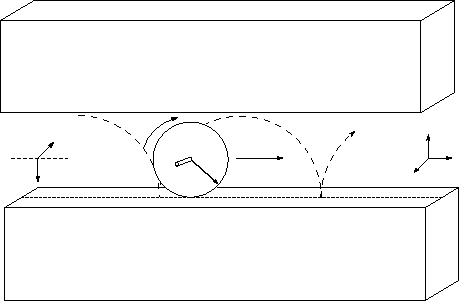
\includegraphics[width=\textwidth]{v3_3}
	\caption{Движение заряда в скрещенных полях}
	\figmark{Crossed fields}
\end{figure}
\todo[inline,author=Popov]{Рисунок странный. Что там по центру? Надо бы нарисовать другой}

Для уяснения идеи метода магнетрона, рассмотрим вначале движение заряда в
<<плоском магнетроне>>, который можно
представить себе в виде плоского конденсатора, помещённого в магнитное поле так,
что $\vec{E}\bot\vec{B}$ (рис.~\figref{Crossed fields}). При этом отрицательная
пластина конденсатора играет роль катода, положительная соответственно анода.
Если бы магнитного поля не было, то все электроны, вылетевшие без начальной
скорости из катода такого плоского диода, попадали бы на анод. При наличии
магнитного поля траектории электронов искривляются, вследствие чего при
достаточно большом магнитном поле ни один электрон не достигнет анода. Для
заданного напряжения между катодом и анодом существует некоторое критическое
значение магнитной индукции~$B_\text{кр}$, при котором траектории касаются
поверхности анода. Если~$B<B_\text{кр}$, то все электроны достигают анода и ток
через магнетрон имеет то же значение, что и без магнитного поля. Если же
$B>B_\text{кр}$, то электроны не достигают анода и ток через лампу равен нулю.

Рассчитаем это критическое значение индукции магнитного поля. Уравнения движения
электрона в нашем случае имеет вид
\begin{equation}
	\eqmark{3.9}
	m\frac{dv_x}{dt}=ev_y B,
\end{equation}
\begin{equation}
	\eqmark{3.10}
	m\frac{dv_y}{dt}=eE-ev_x B
\end{equation}
при начальных условиях $x(0)=y(0)=0$, $v_x(0)=v_y(0)=0$.

Непосредственной подстановкой несложно убедиться в том, что решением системы
дифференциальных уравнений с заданными
начальными условиями является уравнение циклоиды (в параметрической форме):
\begin{equation}
	\eqmark{3.11}
	x = vt - R\sin\omega t,\qquad y = R(1-\cos\omega t),
\end{equation}
где $ v=E/B$, $R=v/\omega=Em/(eB^2)$.

Касание анода происходит при $2R=d$ ($d$~--- расстояние между анодом и катодом).
Этому значению соответствует
критическое поле
\begin{equation}
	B_\text{кр}=\frac{\sqrt{2V}}{d\sqrt{e/m}}.
	\eqmark{3.12}
\end{equation}
Из последней формулы находим удельный заряд:
\begin{equation}
	\eqmark{3.13}
	\frac{e}{m}=\frac{2V}{d^2B_\text{кр}^2}.
\end{equation}
\todo[inline,author=Popov]{Убрать детали в описание работы. Во введении ---
    только общие соотношения}

Эта формула позволяет вычислить~$e/m$, если при заданном значении напряжения на
аноде~$V$ найти такое значение
магнитного поля, при превышении которого ток в магнетроне отсутствует.
\todo[inline,color=cyan]{<---}


\introsection{Электрический ток в вакуумном диоде}

\todo[inline,author=Popov]{Текст написан плохо и изыточно. Можно короче и лучше --->}
Электрический ток в вакуумном диоде представляет собой упорядоченное движение
электронов, испускаемых катодом. Явление испускания электронов поверхностью
твёрдого тела или жидкости называется \term{электронной эмиссией}.
Существует несколько видов электронной эмиссии. В~частности, в случае
испускания электронов поверхностями нагретых тел эмиссия называется
\term{термоэлектронной}.

Для удаления электрона из твёрдого вещества в вакуум необходимо совершить работу.
Работу по переводу электрона в свободное состояние с нулевой кинетической
энергией называют \term{работой выхода}. В~случае термоэлектронной эмиссии
работа выхода совершается за счёт кинетической энергии электронов,
которой они обладают внутри тела. Также работа может быть совершена внешним полем.
У~чистых металлов работа выхода составляет несколько электрон-вольт.

При повышении температуры металла увеличивается энергия теплового движения
электронов, количество быстрых электронов и заметное их количество сможет
преодолеть задерживающее электрическое поле и выйти из металла. Если приложить
электрическое поле, направленное к поверхности металла, то оно будет увлекать
вышедшие электроны и через вакуум потечёт электрический ток.
Этот ток называется \term{термоэлектронным}.

При \important{холодном} катоде ток через диод при подаче на анод
положительного потенциала практически отсутствует. Если же \important{нагреть}
катод, то в диоде возникает заметный ток. Ток прекращается при изменении
полярности батареи. Это как раз и указывает на то, что носителями тока в диоде
являются отрицательно заряженные частицы --- электроны.

Если бы все электроны, вылетающие из поверхности катода, попадали на анод, то
сила термоэлектронного тока~$I$ не зависела бы от величины приложенного
напряжения~$V$. На самом деле это не так. С~возрастанием напряжения ток растёт.
Однако возрастание идёт не пропорционально~$V$, так что закон Ома для вакуумного
диода не выполняется. Нелинейная зависимость тока от напряжения объясняется тем, что в пространстве
между катодом и анодом образуется отрицательный пространственный заряд,
изменяющий распределение потенциала в диоде.

При достижении определённого напряжения дальнейшее
нарастание тока практически прекращается. Ток достигает предельного значения,
называемого \term{током насыщения}. Величина тока насыщения определяется количеством
электронов, которое способно выйти из поверхности катода в единицу времени, и,
следовательно, увеличивается с ростом температуры. Если электрическое поле настолько
сильное, что способно отвести все эмитированные электроны, то дальнейшее
увеличение напряжения уже не приводит к увеличению термоэлектронного тока.
\todo[inline]{<--}

\todo[inline,color=green,author=Popov]{Вставить вместо текста выше -->}
Электрический ток в вакуумном диоде представляет собой упорядоченное движение
свободных электронов, испускаемых катодом. Характерной особенностью
такой системы является наличие в системе пространственного заряда. При этом
электроны, в отличие от обычного проводника, практически не испытывают
сопротивления своему движению. Как следствие, для вакуумного диода
не применим закон Ома.

Явление испускания электронов поверхностью твёрдого тела или жидкости называется
\term{электронной эмиссией}. Для удаления электрона из твёрдого вещества в
вакуум необходимо совершить работу, называемую \term{работой выхода}. По порядку
величины работа выхода составляет несколько электрон-вольт (у чистых металлов).
Один из механизмов эмиссии --- испускание электронов нагретыми телами. Такая
эмиссия называется \term{термоэлектронной}.
Работа выхода при этом совершается за счёт кинетической энергии электронов,
которой они обладают внутри тела.

Если создать электрическое поле вне металла, оно будет увлекать вышедшие
электроны и через вакуум потечёт электрический ток.
С повышением температуры поверхности экспоненциально быстро растёт доля частиц,
способных преодолеть потенциальный барьер и выйти из металла,
и следовательно растёт интенсивность эмиссии электронов. Это приводит к тому, что
в пространстве диода~--- особенно вблизи катода~--- накапливается отрицательный
объёмный заряд, экранирующий внешнее поле. Из-за этого результирующий ток в диоде
оказывается значительно меньше тока эмиссии с катода.
Такой режим работы диода называют \term{режимом объёмного заряда}.

При достижении определённого напряжения дальнейшее нарастание тока практически
прекратится~--- ток достигает предельного значения $I_{нас}$, называемого
\term{током насыщения}. Это обусловлено ограниченностью эмиссионной способности
катода~--- величина тока насыщения определяется количеством электронов,
которое способно выйти из поверхности катода в единицу времени.
\todo[inline,color=green]{<---}


\paragraph{Закон 3/2 для вакуумного диода.}
Рассмотрим режим объёмного заряда в простейшем случае \important{плоского} диода.
Его электроды представимы в виде двух параллельных плоскостей,
между которыми задано напряжение $V$. Расстояние~$d$ между электродами много
меньше их площади. Направим ось~$x$ перпендикулярно к поверхности катода
в сторону анода, совместив начало координат с поверхностью
катода. В~этой модели задача стала одномерной~--- все величины являются
функциями только координаты~$x$.

Запишем для электрического поля теорему Гаусса в дифференциальной форме:
\[
\frac{dE}{dx} = \frac{\rho}{\varepsilon_0},
\]
где~$\rho(x)$~--- плотность электрического заряда. По определению потенциала
электростатического поля имеем
\[
E = -\frac{d\varphi}{dx}.
\]
Отсюда находим, что $\varphi(x)$ удовлетворяет уравнению
\begin{equation}
	\eqmark{3.14}
	\frac{d^2\varphi}{dx^2}=-\frac{\rho}{\varepsilon_0}.
\end{equation}
Это частный (одномерный) случай \term{уравнения Пуассона}.

Плотность тока в диоде равна $j=\rho v$. В стационаре заряд нигде не
накапливается, поэтому плотность тока всюду одинакова: $j=\const$.
Скорость электронов~$v$ можно определить из закона сохранения энергии:
\begin{equation*}
	\frac{mv^2}{2}=e\varphi.
\end{equation*}
Здесь мы пренебрегли \important{начальными тепловыми скоростями},
с которыми вылетают электроны с поверхности катода. Это можно сделать, если
приложенное напряжение достаточно велико: $eV\gg mv_{T}^2/2$. Начало отсчёта
потенциала выбрано на катоде.

Исключив из полученных соотношений плотность электронов~$\rho$ и скорость~$v$,
приходим к уравнению
\begin{equation}
	\eqmark{3.15}
    \frac{d^2\varphi}{dx^2}=\sqrt{\frac{m}{2e\varphi}} \frac{j}{\varepsilon_0}
\end{equation}
с граничными условиями
\begin{equation*}
 \varphi(0)=0,\qquad \varphi(d)=V.
\end{equation*}

Для однозначного решения этого дифференциального уравнения второго порядка
необходимо ещё одно граничное условие.
\todo[inline,author=Popov]{Это неправильное объяснение выбора граничного
    условия! В общем случае решения с конечными $E$ и $j$
на катоде существуют! На самом деле здесь физическое условие бесконечной
эмиссионной способности катода
--->}
 Если сопоставить уравнения \eqref{3.14} и \eqref{3.15}, то можно сделать вывод
об обращении плотности заряда на катоде в бесконечность. Точка~$x=0$ является
особой точкой уравнения \eqref{3.15}, в которой оно теряет смысл. Это связано с
тем, что мы пренебрегли тепловыми скоростями на катоде, приняв их равными нулю.
Оказывается, что в этой модели плотность тока через диод получается конечной,
только если напряжённость поля у катода равна нулю.
Это условие означает, что поле возникающего вблизи катода пространственного заряда полностью экранирует
электрическое поле, создаваемое разностью потенциалов между анодом и катодом.
Таким образом, получаем второе граничное условие в виде
\begin{equation*}
    \left.\frac{d\varphi}{dx}\right|_{x = 0}=0.
\end{equation*}
\todo[inline]{<---}

\todo[inline,author=Popov,color=green]{Вставить этот текст --->}
В общем случае это должна быть связь между плотностью тока~$j$ и электрическим
полем на поверхности катода $E_0 = -\left.\frac{d\varphi}{dx}\right|_{x=0}$,
которую однако  теоретически установить затруднительно.
Учтём, что в режиме объёмного заряда количество электронов, способных покинуть
катод из-за его нагрева, значительно превосходит ток в диоде.
Следовательно, \important{эмиссионная способность катода практически не ограничена},
поэтому чтобы плотность тока оставалась конечной,
напряжённость электрического поля внутри катода нужно устремить к нулю, $E_0\to 0$.
Таким образом, получаем второе граничное условие в виде
\begin{equation*}
    \left.\frac{d\varphi}{dx}\right|_{x = 0}=0.
\end{equation*}

Прямой подстановкой можно проверить, что решением \eqref{3.15},
удовлетворяющим данным граничным условиям, является функция вида
\begin{equation*}
    \varphi^{3/2} =\const \cdot j x^2.
\end{equation*}
Подставляя $\varphi(d)=V$, получим связь между током и напряжением
(вольт-амперную характеристику) в вакуумном диоде:
\begin{equation}
    I \propto V^{3/2}.
\end{equation}
Это так называемый <<\term{закон 3/2}>> \term{Чайлда--Ленгмюра}.

Как следует непосредственно из проведенного вывода,
в реальной системе <<закон 3/2>> нарушается как при слишком малых напряжениях,
когда нельзя пренебрегать начальными тепловыми скоростями электронов,
так и при слишком больших напряжениях, когда диод переходит в режим насыщения.
В~промежуточной области закон хорошо подтверждается на опыте, в том числе
и для электродов неплоской геометрии.
\todo[inline,color=green]{<---}

\todo[inline,author=Popov,color=cyan]{Убрать в описание работы и там дополнить --->}
Теперь задача о распределении потенциала становится однозначной и приводит к
решению
\begin{equation*}
	j=\frac{4\varepsilon_0}{9x^2}\sqrt{\frac{2e}{m}}\varphi^{3/2}.
\end{equation*}
\todo[inline,author=Popov]{Убрать детали в описание работы,
во введении --- только общие законы}

Так как $\varphi(d)=V$, где~$d$~--- расстояние между электродами, то для
зависимости тока от напряжения получаем
\begin{equation*}
	I=\frac{4\varepsilon_0 S}{9d^2}\sqrt{\frac{2e}{m}}V^{3/2},
\end{equation*}
где~$S$~--- площадь катода. Мы получили зависимость тока через плоский диод от
приложенного к нему напряжения, известную как <<закон трёх вторых>> для плоского
диода. Оказывается, что не только для плоского вакуумного диода, а и для
вакуумного диода с электродами любой другой геометрии ток подчиняется <<закону
степени трёх вторых>>.

Полученная формула подсказывает процедуру измерения удельного заряда электрона.
Для этого достаточно по
результатам эксперимента построить график зависимости тока от напряжения в
степени трёх вторых, который должен
представлять собой прямую линию, проходящую через начало координат. Угол наклона
этой прямой линии пропорционален (с известным коэффициентом) квадратному корню
из~$e/m$~--- искомой величины удельного заряда электрона.
\todo[inline,color=cyan]{<---}

\introsection{Свободные носители заряда в металлах и~полупроводниках}

Проводимость большинства твёрдых тел связана с движением электронов. Электроны
входят в состав атомов всех тел, однако одни тела не проводят электрический ток
(диэлектрики), а другие являются хорошими его проводниками. Причина различия
заключается в особенностях энергетического состояния внешних электронов атомов в
этих веществах.

При объединении атомов в твёрдое тело (кристалл) внешние электроны теряют связь
со <<своими>> атомами и теперь принадлежат всему кристаллу в целом. Каждому
уровню энергии электрона одиночного атома соответствует в кристалле группа
близких по энергии уровней (разрешённая зона), в которой число уровней равно
числу мест на соответствующем атомном уровне, умноженному на число атомов в
кристалле. Число уровней, объединившихся в зону, при слиянии не меняется. Оно
определяет максимальное число электронов, которое может <<поместиться>> в зоне
(в силу принципа Паули).

Если одна из энергетических зон до конца заполнена электронами, а следующая зона
совершенно пуста, то под действием слабого внешнего электрического поля
электронам некуда перетекать, и вещество является \important{диэлектриком}.
Верхняя из заполненных зон называется \important{валентной зоной}.

Положение меняется, если в кристалле имеется зона, частично заполненная
электронами. В~этом случае внешнее электрическое поле может изменить
распределение электронов по уровням энергии и создать упорядоченное движение
электрических зарядов. Частично заполненная зона называется \important{зоной
проводимости}. Частично заполненная электронами зона имеется у всех твёрдых
проводников электрического тока; в том числе её имеют все металлы.

Если ширина запрещённой зоны относительно невелика, тепловое движение
перебрасывает часть электронов из валентной зоны в свободную~--- зону
проводимости. При этом в зоне проводимости появляются электроны, а в валентной
зоне~--- свободные места~--- \important{дырки}. Электроны в зоне проводимости и
дырки валентной зоны участвуют в переносе заряда. Такие вещества называются
\important{полупроводниками}. Обычно к полупроводникам относят материалы с
шириной запрещённой зоны $\Delta E \lesssim 2$~эВ. Число носителей тока в
полупроводниках экспоненциально увеличивается с~повышением температуры.

Рассматривая коллективное движение электронов почти заполненной зоны, полезно
мысленно заполнить свободные места
воображаемыми парами, состоящими из электронов с одинаковыми по величине
положительным и отрицательным зарядами. Обычныеотрицательные заряженные
электроны заполняют теперь все уровни и, следовательно, не могут принимать
участия в проводимости. Они образуют структуру, характерную для изоляторов.
Проводимость связана только с введёнными нами
<<электронами>>, обладающими положительным зарядом. Такие <<электроны>> носят
название \important{дырок}. При рассмотрении явлений, происходящих в~металлах
с~почти заполненной валентной зоной, удобно представлять себе дело так, как если
бы проводниками тока были не настоящие электроны, а положительно заряженные
дырки. В~этом случае говорят о \important{дырочном типе проводимости.}

Электронным типом проводимости обладает большинство чистых металлов. Однако в
ряде металлов (бериллий, кадмий и
некоторые другие) основными носителями электрического тока являются дырки. Это
связано с особенностями их зонной
структуры.

\introsubsection{Эффект Холла}

Рассмотрим прохождение тока в рамках модели свободных электронов.
Закон Ома в дифференциальной форме выражает связь векторов~$j$~--- плотности тока
и~$E$~--- электрического поля:
\begin{equation}
	j=\lambda E.
	\eqmark{3.16}
\end{equation}

В~нулевом магнитном поле, если проводящая среда изотропна (то есть не имеет
выделенных направлений), проводимость~$\lambda$ является числом (скаляром). Это
значит, что векторы~$j$ и~$E$ сонаправлены. В~общем же случае
$\widehat{\lambda}$ является тензором второго ранга, то есть матрицей, при
умножении которой на вектор~$E$ получается вектор~$j$. В~присутствии магнитного
поля эта матрица становится недиагональной в результате эффекта Холла. Тензор
удельного сопротивления~$\widehat{\rho}$ является обратным к тензору
проводимости: $E=\widehat{\rho}j$, то есть
$\widehat{\rho}=\widehat{\lambda}^{-1}$.
\todo[inline,author=Popov]{Как-то слишком резко --- бац и тензор. Нужно
    дать более гуманное введение в тему}

Электроны в металлах и легированных полупроводниках движутся с большими
скоростями во всех направлениях, а под действием тянущего
электрического поля приобретают ненулевую среднюю скорость дрейфового движения
$v_{dr}=  Eb$, где~$b$~--- подвижность.

\todo[inline,author=Popov]{Дать чёткое определение эффекту Холла и
    магнито(или магнето?)-сопротивлению}
Разберем магнитосопротивление и эффект Холла на микроуровне. Если магнитное поле
направлено вдоль тока, то
оно не влияет на ток, поскольку сила Лоренца равна нулю. Поэтому мы рассмотрим
случай, когда поле перпендикулярно
току. Пусть рассматриваемая система для простоты содержит носители только одного
сорта (большинство металлов
являются хорошими примерами).
\begin{figure}[h!]
	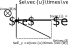
\includegraphics[width=0.9\textwidth]{Chapter_3/Hall_forces}
	\caption{Силы, действующие на носитель заряда в проводящей среде в тянущем
электрическом и перпендикулярном ему магнитном полях.}
	\figmark{Hall forces}
\end{figure}

Если в системе локально течет ток электронов $j_x=nev_{dr\, x}$, направленный
вдоль оси~$x$, а магнитное поле~$B$ направлено вдоль оси~$z$, то на заряды
действует действует сила Лоренца $ F_{L}=e[v_{dr}B]$ вдоль оси~$y$.
Сила Лоренца должна приводить к образованию компоненты тока вдоль оси~$y$, но по
условиям ток течет вдоль~$x$. Это значит, что заряды должны перераспределиться
таким образом, чтобы полностью скомпенсировать силу
Лоренца, создав в~$y$ направлении электрическое холловское поле $E_y=v_{dr}B$.
Поскольку сила Лоренца
оказывается полностью скомпенсирована $eE_y$, то электрон движется так, как если
бы магнитного поля не
было, то есть $j_x=E_xbne$, $j_y=j_z=0$. Это позволяет написать в явном виде
тензор удельного сопротивления:
\begin{equation}
	\widehat{\rho}(B)=\frac{1}{bne}\left(
	\begin{tabular}{ccc}
		{\it 1} & {\it bB} & {\it 0} \\
		{\it -bB} &{\it 1}& {\it 0} \\
		{\it 0} &{\it 0}& {\it 1}\\
	\end{tabular}
	\right).
	\eqmark{3.17}
\end{equation}

Здесь коэффициент, стоящий перед матрицей,
\begin{equation}
	\frac{1}{bne} = \rho_0
	\eqmark{UdSoprot}
\end{equation}
есть удельное сопротивление полупроводника при отсутствии магнитного поля.

Обращением этой матрицы нетрудно получить тензор проводимости:
\begin{equation}
	\widehat{\lambda}(B)=\frac{bne}{1+b^2B^2}\left(
	\begin{tabular}{ccc}
		{\it 1} & {\it bB} & {\it 0} \\
		{\it -bB} &{\it 1}& {\it 0} \\
		{\it 0} &{\it 0}& {\it 1}\\
	\end{tabular}
	\right).
	\eqmark{3.18}
\end{equation}

Существуют две основных и принципиально различных геометрии для исследования
магнитосопротивления: геометрия
мостика Холла и геометрия диска Корбино (см. рис.~\figref{Geometries}).

В~геометрии мостика Холла ток вынуждают течь вдоль образца, сила Лоренца
прибивает носители к краю образца, создавая тем самым холловское поле, которое
компенсирует силу Лоренца. Напряжение между точками $V_{xy}$ равно~$E_yw$, где,
согласно уравнению \eqref{3.17}, $E_y=\rho_{yx}\times j_x=j_x B/(ne)$. Плотность
тока, текущего через образец, равна полному току~$I$, деленному на площадь
поперечного сечения образца~$wh$. Таким образом, для холловского напряжения
имеем:
\begin{equation}
	V_{xy}=\frac{IB}{neh}.
	\eqmark{3.19}
\end{equation}

В~этой же модели для падения напряжения вдоль образца имеем:
\begin{equation}
	V_{xx}=\frac{Il}{nebwh}.
	\eqmark{3.20}
\end{equation}

Tаким образом, удельное сопротивление~$\rho_{xx}$ образца не зависит от
магнитного поля (магнитосопротивление равно 0). Этот факт объясняется тем, что
сила Лоренца и сила ЭДС Холла (рис. \figref{Hall forces}) полностью
уравновешивают друг друга. В~реальных системах, тем не менее, предположения
модели не выполняются и магнитосопротивление зачастую отлично от 0. Причины
могут быть различными:
\begin{enumerate}
\item Система может быть анизотропной, то есть в разных направлениях ($x,y,z$)
токопроводящие свойства различны. В~этом случае величина силы Лоренца содержит
не среднюю дрейфовую скорость, а зависит от направления большой мгновенной
скорости электрона.

\item Система может быть многокомпонентной. Например, в полупроводниках часто
одновременно существуют электроны и дырки, концентрации ($n$ и~$p$) и
подвижности ($b_n$ и~$b_p$) которых в общем случае различаются. Тогда полный
тензор проводимости будет суммой тензоров проводимости двух компонент вида
\eqref{3.18}. Обращением тензора проводимости в пределе малых магнитных полей
можно показать, что холловское сопротивление двухкомпонентной системы в
полупроводнике равно:
\begin{equation}
	R_{xy}\equiv \frac{V_{xy}}{I}=\frac{n{b_n}^2-p{b_p}^2}{eh(nb_n+pb_p)^2}B
	\eqmark{3.21}
\end{equation}

\item Существуют квантовые эффекты в проводимости, которые приводят к тому, что
подвижность зависит от магнитного поля. Например если сам проводящий материал
является ферромагнетиком, то с ростом поля он намагничивается, количество
доменов уменьшается, а доменные стенки являются причиной сильного рассеяния, то
есть уменьшают подвижность.
\end{enumerate}

Поскольку холловское сопротивление содержит толщину образца~$h$, то договорились
называть холловское сопротивление, умноженное на толщину образца, постоянной
Холла. Постоянная Холла характеризует материал, так как зависит только от
концентрации носителей в нем:
\begin{equation}
	R_x=\frac{1}{ne}
	\eqmark{HallConstant}
\end{equation}
или от соотношений между концентрациями и подвижностями, если в материале
несколько типов носителей. В~таблице в приложении даны постоянные Холла для
различных металлов. Для полупроводников постоянные Холла сильно зависят от
наличия малых концентраций примеси и температуры.

Отдельно следует упомянуть, что существуют двумерные системы (например, графен),
в которых движение носителей заряда происходит только в плоскости, а движение в
перпендикулярном направлении квантовомеханически запрещено. В~этих системах
концентрация измеряется в количестве носителей на единицу площади, а холловская
постоянная есть просто холловское сопротивление, делённое на магнитное поле. В
двумерных системах тензоры в формулах \eqref{3.17} и \eqref{3.18} содержат
только~$x$ и~$y$ компоненты, то есть являются матрицами~$2\times2$.
\todo[inline, author=Popov]{А стоило ли отдельно упоминать графен,
    прерывая повествование? Лирические
    отступления вынести в конец или в начало раздела}

Измерения в геометрии мостика Холла представляют собой четырехконтактные
измерения, то есть два контакта используются для задания тока через образец, а с
двух контактов снимается падение напряжения. Поскольку вольтметр обладает
бесконечным сопротивлением (то есть ток через него не течет), измеряемое падение
напряжения совершенно не зависит от свойств контактов, а определяется только
свойствами материала.

Геометрия диска Корбино представляет собой двухточечную схему, то есть
сопротивление образца в ней суммируется с сопротивлениями контактов. Поэтому
исключительно важно создать низкоомные контакты к образцу, сопротивлением
которых можно пренебречь. В~геометрии Корбино из-за аксиальной симметрии не
формируется холловское напряжение. Электрическое поле направлено строго по
радиусу системы. В~магнитном поле ток вынужден протекать под углом к
электрическому полю, то есть по спирали. Из-за симметрии полный ток включает
только компоненту вдоль радиуса $j_r=\lambda_{xx} E_r$. Плотность тока может
быть выражена через полный ток и толщину образца $j_r=I/(2\pi rh)$.
Теперь запишем для напряжения:
\begin{equation*}
V={\int_{r_1}}^{r_2}E_r dr={\int_{r_1}}^{r_2}\frac{j_r}{\lambda_{xx}}
dr={\int_{r_1}}^{r_2}I\rho_0\frac{1+b^2B^2}{2\pi
rh}dr=I\rho_0\frac{1+b^2B^2}{2\pi h}\ln{\frac{r_2}{r_1}}.
\end{equation*}
\todo[inline,author=Popov]{Убрать этот ужас в описание работы}

Если система однокомпонентная, то магнетосопротивление в геометрии Корбино есть
\begin{equation}
	R(B) = R_0(1+b^2B^2)
	\eqmark{MagnetoSoprot}.
\end{equation}

Здесь
\begin{equation}
	R_0 = \frac{\rho_0}{2\pi h} \ln{\frac{r_2}{r_1}}
	\eqmark{KorbinoSoprot}
\end{equation}

Для наблюдения этого магнитосопротивления выбирают систему с большой подвижнотью
носителей (как правило, это полупроводник с низкой эффективной массой электронов
типа InSb).

\begin{figure}[h!]
	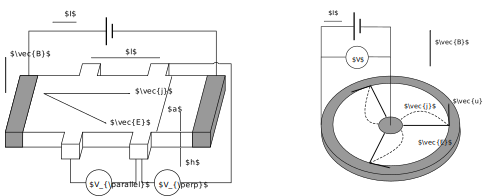
\includegraphics[width=0.9\linewidth]{Chapter_3/2schemes}
	\caption{Две геометрии для исследования влияния магнитного поля на
проводящие свойства: мостик Холла (слева) и диск Корбино (справа).}
	\figmark{Geometries}
\end{figure}

При наложении внешнего электрического поля~$E$ электроны начинают ускоряться.
Однако после некоторого <<свободного пробега>> происходит соударение с решёткой,
электрон теряет набранную энергию, и процесс ускорения начинается заново.
Соударения с решёткой, подобно вязкому трению, приводят к тому, что
результирующее движение электрона можно описать некоторой средней скоростью
$\left< v \right>$, пропорциональной внешнему полю:
\begin{equation}
	\eqmark{3.22}
	\left< \vec{v} \right>=-b\vec{E}.
\end{equation}

\todo[inline,author=Popov]{Что это? Куски старого текста? Раздел остро
    нуждается в редактировании!}

Введённая здесь величина~$b$ называется \important{подвижностью}. В~определённых
пределах изменения температуры,
напряжённости поля и его частоты эта характеристика вещества остаётся постоянной
и приводится в справочниках. Для
положительно заряженных носителей тока в формуле \eqref{3.22}, очевидно, стоит
знак <<плюс>>.

При установившемся движении средняя сила, действующая на электроны со стороны
кристаллической решётки, равна внешней силе~$-eE$ и направлена в противоположную
сторону. Поэтому действие кристаллической решётки на движение электронов в
среднем эквивалентно силе трения, пропорциональной скорости:
\begin{equation}
	\eqmark{3.23}
	F_\text{тр}=-\frac{e}{b}\average{\vec{v}}.
\end{equation}

Если концентрация электронов равна~$n$, величина плотности тока определится
очевидным соотношением
\begin{equation}
	\eqmark{3.24}
	j=en\average{v}=enbE.
\end{equation}

Таким образом, выполняется закон Ома~--- величина плотности тока~$j$
пропорциональна напряжённости поля~$E$:
\begin{equation}
	\eqmark{3.25}
	j=\sigma E.
\end{equation}

Сравнивая \eqref{3.24} и \eqref{3.25}, получаем выражение для проводимости
\begin{equation}
	\eqmark{3.26}
	\sigma=enb.
\end{equation}

Химически чистые полупроводники обладают проводимостью, которая связана с
небольшим числом электронов в зоне
проводимости и таким же числом дырок в валентной зоне. Такая проводимость
называется собственной~--- она не связана с примесями. Добавление небольшого
количества специально подобранных примесей (так называемое
легирование) может существенно увеличить проводимость полупроводников или даже
создать ощутимую проводимость при комнатной температуре в веществах с
запрещённой зоной, ширина которой заметно превышает 2~эВ. Такое происходит,
когда атомы примеси имеют энергетические уровни в запрещённой зоне основного
материала.

Если заполненные примесные уровни расположены вблизи потолка запрещённой зоны,
находящиеся на этих уровнях электроны легко переходят в зону проводимости.
Наоборот, на свободные уровни у дна зоны проводимости легко переходят электроны
валентной зоны с образованием в этой зоне дополнительного количества дырок. В
обоих случаях число переносчиков заряда увеличивается, и проводимость
возрастает. В~первом случае говорят о полупроводниках \important{электронного},
или $n$-типа, а во втором~--- о  полупроводниках дырочного, или $p$-типа. В
общем случае в процессе электрической проводимости участвуют как электроны, так
и дырки. Удельная электрическая проводимость полупроводника при этом равна
\begin{equation}
	\eqmark{3.27}
	\sigma=e(nb_e+pb_p),
\end{equation}
где~$n$ и~$p$~--- концентрации электронов и дырок, а~$b_e$ и~$b_p$~--- их
подвижности. В~случае \important{примесной
проводимости} один тип носителей обычно существенно преобладает над другим и в
формуле \eqref{3.27} можно пренебречь одним из слагаемых.



\begin{lab:literature}
	\item{ \emph{Сивухин Д.В.} Общий курс физики.~--- T.~III. Электричество.~---
М.: Наука, 1983. \S\S~86, 95, 98, 100.}
	\item{ \emph{Кингсеп А.С., Локшин Г.Р., Ольхов О.А.} Основы физики.
Т.~1.~--- М.: Физматлит, 2001. \S\S~8.1--8.3.}
\end{lab:literature}




\newpage

\lab{Измерение удельного заряда электрона методами магнитной фокусировки и
магнетрона}

\aim{определение отношения заряда электрона к его массе методом магнитной
фокусировки и методом магнетрона.}

\equip{А)~электронно-лучевая трубка (с блоком питания), соленоид, 
    регулируемый источник постоянного тока, вольтметр, 
    магнитометр (миллитесламетр или милливеберметр);
Б)~электронная лампа с цилиндрическим анодом, 
регулируемый источник постоянного тока, соленоид, вольтметр, два амперметра.}

Перед выполнение работы необходимо ознакомиться с теоретическим введением
к Разделу (п. \ref{sec:freemotion}).

\labsection{А.~Метод магнитной фокусировки}

В постоянном однородном магнитном поле траектории заряженных частиц представляют
собой спирали, радиус которых определяется формулой \chaptereqref{3.4}.
За время $T_B= \frac{2\pi r_B}{v_{\perp}}$, которое можно назвать
\mbox{\term{циклотронным периодом}}, заряд сместится вдоль магнитного поля на 
расстояние $L$ (шаг спирали):
\begin{equation}
    \eqmark{3.6}
    L = v_{\parallel}T_B =\frac{2\pi v\cos\alpha}{\frac{e}{m}B},
\end{equation}
где $\alpha$ --- угол между вектором скорости $\vec{v}$ и направлением поля $\vec{B}$.
Если углы малы, $\alpha \ll 1$, то $\cos\alpha \approx 1$ и
\begin{equation}
    \eqmark{3.7}
    L \approx \frac{2\pi v}{\frac{e}{m}B}.
\end{equation}
Таким образом, при малых углах расстояние~$L$ не зависит от~$\alpha$, так
что все электроны, вышедшие из одной точки, после одного оборота вновь соберутся
в одной точке~--- \emph{сфокусируются}. Как следует из \eqref{3.7}, 
индукция поля~$B$, при которой точка фокусировки отстоит от точки вылета 
на расстоянии~$L$, определяется величиной~$e/m$~--- 
\term{удельным зарядом частицы}.

%В работе исследуется пучок электронов, создаваемый электронно-лучевой трубкой, 
%помещённой в магнитное поле соленоида.
%Скорость движения электрона задаётся разностью потенциалов~$U$,
%пройденной им до попадания в область магнитного поля:
%\begin{equation*}
%  \frac{mv^2}{2}=eU,
%\end{equation*}
%откуда
%\begin{equation}
%  \eqmark{3.3}
%  v=\sqrt{\frac{2eU}{m}}.
%%   = 6\cdot10^5\sqrt{V}~\frac{m}{c}.
%\end{equation}
%
%Пусть $B_{ф}$ --- индукция поля, при которой достигается фокусировка.
%Из \eqref{3.3} и \eqref{3.7} выразим удельный заряд электрона~$e/m$
%через $B_{ф}$:
%\begin{equation}
%\eqmark{3.8}
%\frac{e}{m}=\frac{8\pi^2 U}{L^2B_{ф}^2}.
%\end{equation}
%Эта формула и лежит в основе экспериментального измерения удельного заряда
%электрона \important{методом магнитной фокусировки}.

\experiment 

Основной частью установки является электронный осциллограф, трубка
которого вынута и установлена в длинном соленоиде, создающем магнитное поле,
 направленное вдоль оси трубки. Вылетая с катода, электроны имеют, вообще говоря, 
 разные начальные скорости, соответствующие тепловой энергии $\sim 0,1\;эВ$.
Затем эмитированные катодом электроны ускоряются большой анодной 
разностью потенциалов $U_А~\sim 1\;кВ$ и пропускаются 
через две диафрагмы, благодаря чему получается пучок частиц с малой расходимостью
($\Delta \alpha \ll 1$) и малым разбросом продольных скоростей 
около значения
\[
v_{\parallel}=\sqrt{\frac{2eU_А}{m}},
\]
следующего из закона сохранения энергии.

В магнитном поле соленоида коллимированные электроны будут двигаться 
по спиралям практически с одним и тем же шагом~$L$
(см. формулу \eqref{3.6}), и, следовательно, будут встречаться вновь, 
пересекая ось пучка на расстояниях~$nL$, $n=1,\,2,\,3,\ldots$
В~этих точках сечение пучка будет наименьшим, и при изменении магнитного 
поля изображение пучка на экране будет периодически стягиваться 
в ярко светящуюся точку. 
Таким образом, удельный заряд может быть получен из соотношения
\begin{equation}
\frac{e}{m}=\frac{8\pi^2U}{L^2}\cdot\frac{n^2}{B_ф^2(n)}.
\eqmark{3.1.1}
\end{equation}
Эта формула и лежит в основе экспериментального измерения удельного заряда
электрона \important{методом магнитной фокусировки}.


Анодное напряжение, определяющее продольную скорость электронов, измеряется
вольтметром. Магнитное поле в соленоиде создаётся постоянным током
(рис.~\figref{Magnetic focusing scheme}), величина которого задаётся источником
питания постоянного тока и измеряется амперметром~A источника. Ключ~К
служит для изменения направления поля в соленоиде.

\begin{figure}[h]
    \centering\small
    \pic{5.1cm}{Chapter_3/3_1_1}
    \caption{Схема измерений по~методу магнитной фокусировки}
    \figmark{Magnetic focusing scheme}
\end{figure}

Величина магнитного поля определяется с помощью магнитометра, датчик которого
расположен внутри соленоида. В~качестве магнитометра может использоваться
\emph{милливеберметр} (\emph{флюксметр}). Датчиком милливеберметра является 
измерительная катушка, намотанная на один каркас с соленоидом. 
Таким образом измеряется изменение магнитного потока,
пронизывающего измерительную катушку. Описание милливеберметра и правила работы
с ним приведены на с.~\pageref{MWB}. Альтернативно индукция поля может измеряться
\emph{миллитесламетром} (\emph{датчиком Холла}).

На точность результатов может влиять внешнее магнитное поле, особенно
продольное. Оно не вызывает размытия фокуса, но изменяет величину фокусирующего
поля. Присутствие внешнего магнитного поля проще всего обнаружить с помощью
переполюсовки соленоида: при изменении направления поля показания
милливеберметра будут отличаться, но их полусумма не зависит от наличия
постоянного продольного поля.

Измерение магнитного поля производится в предварительных опытах: 
при отключенном ключе~К устанавливается связь между силой тока, протекающего 
через соленоид, и индукцией магнитного поля в соленоиде. 
По измеренным значениям строится \emph{калибровочный график} $B(I)$, 
который используется при обработке результатов
основных измерений для определения индукции магнитного поля по известному току.

\begin{lab:task}

\taskpreamble{Измерьте значения магнитных полей, при которых происходит 
    фокусировка электронного пучка. По результатам измерений рассчитайте 
    удельный
заряд электрона $e/m$.}
    
\item Ознакомьтесь с назначением ручек источника питания и с устройством 
    используемого в работе магнитометра. 
    
\item Проведите измерение калибровочной кривой $B(I)$ --- зависимости магнитного поля
в соленоиде от тока в его обмотке. В~случае использования установки с
милливеберметром поле~$B$ вычисляется через поток $\Phi=BSN$, пронизывающий пробную
катушку (значение параметра~$SN$ катушки указано на установке).

Проведите измерения во всём доступном диапазоне изменения тока при двух
направлениях тока через обмотку.

\item При минимальном или нулевом токе через соленоид включите осциллограф и
подайте напряжение с внешнего генератора на вертикальный 
вход усилителя. На экране появится светящаяся линия.

%\todo[inline,author=Popov]{Уточнить, что за генератор и куда подавать}

\item Постепенно увеличивая ток через соленоид, найдите значение тока~$I_ф$, при
котором линия в первый раз стягивается в точку 
(сила тока~$I_ф$ зависит от ускоряющего напряжения~$U_А$, 
которое в свою очередь пропорционально 
яркости луча, поэтому \emph{не следует менять настройку яркости до конца измерений}).

Продолжая увеличивать ток, получите зависимость~$I_ф(n)$ от порядкового номера
фокуса~$n$.

\item Повторите измерения $I_ф(n)$ для обратного направления магнитного поля
в соленоиде.

\item Запишите значение ускоряющего напряжения~$U_А$, длину трубки
$L$ и характеристики приборов.

\item Установите регуляторы источника питания на минимум и выключите его. 
Выключите осциллограф.

\tasksection{Обработка результатов}

\item Постройте калибровочный график $B(I)$.

\item Пользуясь графиком $B(I)$, определите усреднённые значения~$B_ф$ для каждого
фокуса и постройте график зависимости $B_ф(n)$ фокусирующего поля от номера $n$. 
Используйте наклон графика для расчёта~$e/m$ с помощью формулы~\eqref{3.1.1}.

\item Оцените погрешности и сравните результат с табличным.

\end{lab:task}


\labsection{Б. Измерение ${e/m}$ методом магнетрона}

В~так называемом {\important{методе магнетрона}} отношение~$e/m$ измеряется на
основе исследования движения электрона в скрещенных (перпендикулярных друг другу) 
электрическом и магнитном полях. Название метода связано с тем, что такая
конфигурация полей реализуется в \emph{магнетронах}~--- 
генераторах электромагнитных колебаний сверхвысоких частот.

\begin{figure}[h!]
    \centering
    \pic{8cm}{Chapter_3/v3_3}
    \caption{Движение заряда в скрещенных полях (без начальной скорости)}
    \figmark{Crossed fields}
\end{figure}
%\todo[inline,author=Popov]{Рисунок странный. Что там по центру? Надо бы
%    нарисовать другой}

Для уяснения идеи метода магнетрона рассмотрим вначале упрощённую
задачу о движение заряда в <<плоском магнетроне>>. 
Пусть имеется плоский конденсатор, в пространстве между пластинами которого создан
высокий вакуум (вакуумный диод). Поместим его в однородное магнитное поле (например,
внутрь соленоида) так, что $\vec{E}\perp\vec{B}$ (рис.~\figref{Crossed fields}). 
При этом отрицательная пластина конденсатора играет роль катода, 
положительная~--- анода. Если бы магнитного поля не было, то все электроны, 
вылетевшие без начальной скорости из катода, попадали бы на анод. 
При наличии же магнитного поля траектории электронов искривляются, 
вследствие чего при достаточно большом $B$ ни один электрон не достигнет анода.
Таким образом, при
заданном напряжения $V$ между пластинами существует некоторое критическое
значение магнитной индукции~$B_\text{кр}(V)$, при котором траектории касаются
поверхности анода. Если~$B<B_\text{кр}$, то все электроны достигают анода, и ток
через магнетрон имеет то же значение, что и без магнитного поля. Если же
$B>B_\text{кр}$, то электроны не достигают анода, и ток через вакуумный диод равен нулю.

Рассчитаем критическое магнитное поле для плоского конденсатора.
Движение электрона будет иметь характер электрического дрейфа. 
Если начальная скорость равна нулю 
(начальные условия $x(0)=y(0)=0$, $v_x(0)=v_y(0)=0$), 
то, как следует из уравнений \chaptereqref{3.9}, 
траектория частицы будет \emph{циклоидой}:
\begin{equation}
\eqmark{3.11}
x = Vt - R\sin \omega_B t,\qquad y = R(1-\cos\omega_B t),
\end{equation}
где $V=E/B$ --- дрейфовая скорость, $R=V/\omega_B=Em/(eB^2)$.
Касание анода происходит при $2R=h$ ($h$~--- расстояние между анодом и катодом).
Этому значению соответствует критическое поле
\begin{equation}
B_\text{кр}=\frac{\sqrt{2U}}{h\sqrt{e/m}},
\eqmark{3.12}
\end{equation}
где $U=Eh$ --- напряжение между пластинами.
Отсюда находим удельный заряд:
\begin{equation}
\eqmark{3.13}
\frac{e}{m}=\frac{2U}{B_\text{кр}^2h^2}.
\end{equation}

Формула \eqref{3.13} позволяет вычислить~$e/m$, если при заданном 
значении напряжения на диоде~$U$ найти такое значение
магнитного поля, при превышении которого ток в магнетроне отсутствует.

\experiment

В данной работе движение электронов случае происходит в кольцевом пространстве,
ограниченном катодом и анодом двухэлектродной электронной вакуумной лампы 
(рис.~\figref{Two-electrode lamp}).
Нить накала лампы (катод) располагается вдоль оси цилиндрического анода, так что
электрическое поле между катодом и анодом имеет \emph{радиальное} направление. 
Лампа помещается внутри соленоида, создающего магнитное поле, \emph{параллельное оси} лампы.

\begin{figure}[h!]
    \begin{minipage}[b]{0.4\textwidth}
        \centering
        \pic{4cm}{Chapter_3/3_1_2}
        \caption{Схема устройства двухэлектродной лампы}
        \figmark{Two-electrode lamp}
    \end{minipage}
    \hfill
    \begin{minipage}[b]{0.5\textwidth}
        \centering
        \pic{5cm}{Chapter_3/3_1_3}
        \caption{Траектории электронов, вылетающих из~катода, при~разных
            значениях индукции магнитного~поля}
        \figmark{Path of electrons}
    \end{minipage}
\end{figure}

Таким образом, реализуется геометрия скрещенных полей $\vec{E}$ и $\vec{B}$.
Поскольку поле $\vec{E}$ в данном случае не является однородным (оно зависит от расстояния
до оси), траектории частиц будут несколько отличаться от рассмотренного выше плоского
случая. Тем не менее, все качественные особенности траектории сохранятся, а
выражение для критического поля будет отличаться от \eqref{3.13} только
численным коэффициентом порядка единицы.
Подробно задача о движении электронов в такой лампе рассмотрена 
в Приложении к работе, где получено следующее
выражение для удельного заряда:
\begin{equation}
	\frac{e}{m}=\frac{8U_{А}}{B_\text{кр}^2r_{А}^2},
	\eqmark{3.1.3}
\end{equation}
где $r_{А}$~--- радиус анода.

До сих пор мы рассматривали идеальный случай: при $B<B_\text{кр}$ все
электроны без исключения попадают на анод, а при $B>B_\text{кр}$ все они
возвращаются на катод, не достигнув анода. Анодный ток~$I_{А}$ с увеличением
магнитного поля изменялся бы при этом так, как это изображено штриховой линией 
на рис.~\figref{Anode current from induction}. В~реальных условиях
невозможно обеспечить полную коаксиальность анода и катода, вектор индукции
магнитного поля всегда несколько наклонён по отношению к катоду, магнитное поле
не вполне однородно и т.~д. Всё это приводит к сглаживанию кривой 
$I_{А}(B)$ (сплошная линия на рис.~\figref{Anode current from induction}).
Тем не менее, в~хорошо собранной установке перелом функции~$I_A(B)$ остаётся
достаточно резким и может быть использован для измерения~$e/m$.

\begin{figure}[h]
    \centering
    \pic{7cm}{Chapter_3/3_1_4}
    \caption{Зависимость анодного тока от индукции магнитного поля в соленоиде}
    \figmark{Anode current from induction}
\end{figure}

Схема установки изображена на рис.~\figref{Scheme}. 
Анод лампы состоит из трёх немагнитных металлических 
цилиндров одинакового диаметра.
Два крайних цилиндра электрически изолированы от среднего небольшими зазорами и
используются для устранения краевых эффектов на торцах среднего цилиндра, ток с
которого используется при измерениях. В~качестве катода используется тонкая
(диаметр $2r_{К}=50~\text{мкм}$) натянутая вольфрамовая проволока, расположенная по оси
всех трёх цилиндров анодной системы. Катод разогревается проходящим 
через него переменным током (\emph{лампа прямого накала}),
создаваемым стабилизированным источником питания. 
На анод лампы подаётся постоянное напряжение от регулируемого источника, 
измеряемое вольтметром~$V_{А}$. Ток~$I_{А}$ через среднюю секцию анода  
измеряется с помощью миллиамперметра.

\begin{figure}[h]
    \centering
	\pic{6cm}{Chapter_3/3_1_5}
	\caption{Схема измерительной установки}
	\figmark{Scheme}
\end{figure}

Лампа закреплена в соленоиде. Ток $I_{С}$, проходящий через соленоид, подаётся от
независимого источника и измеряется амперметром. Индукция магнитного поля в
соленоиде рассчитывается по току, протекающему через обмотку соленоида.
Коэффициент пропорциональности между ними указан на установке.


\begin{lab:task}

\taskpreamble{В~работе предлагается исследовать зависимость анодного тока от магнитного
поля в соленоиде при различных напряжениях на аноде лампы.
По результатам измерений --- рассчитать удельный заряд электрона.}

    
\item Установите минимальный потенциал~$U_{А}$ на аноде лампы, 
рекомендуемый в описании установки. Измерьте зависимость анодного тока~$I_A$ 
от тока через соленоид $I_{С}$. В~области резкого изменения тока
экспериментальные точки должны располагаться чаще 
(см. рис.~\figref{Anode current from induction}).

\item Измерьте аналогичные зависимости $I_{А}(I_{С})$ для 6--8 
значений анодного напряжения~$U_{А}$ в диапазоне, указанном в описании установки.

\item Запишите параметры установки и характеристики приборов. 

\item Установите регуляторы источников питания на минимум и отключите
источники от сети.

\tasksection{Обработка результатов}

\item Постройте семейство зависимостей анодного тока от магнитного поля $I_{A}(B)$ 
для всех значений $U_{А}$. 

\item По участкам графика с максимальным наклоном для каждого значения~$U_{А}$ 
определите критическое значение индукции магнитного поля~$B_\text{кр}$.

\item Постройте  график зависимости~$B_\text{кр}^2$ от~$U_{А}$. 
Убедитесь, что зависимость является линейной. Используя
формулу \eqref{3.13}, по угловому коэффициенту полученной 
прямой определите удельный заряд электрона~$e/m$.

\item Оцените погрешности. Сравните результат с табличным.

\end{lab:task}


\begin{lab:questions}
\item Что такое циклотронная частота и ларморовский радиус?
\item Что такое дрейф в скрещенных полях? 
Чем определяется и куда направлена дрейфовая скорость?
\item Что представляет собой траектория движения частицы без начальной скорости 
в однородных скрещенных электрическом и магнитном полях?
\item При каких условиях возможна фокусировка пучка электронов внешним 
магнитным полем?
\item Получите выражение для критического магнитного поля~$B_{кр}$ 
в методе магнетрона
с плоскими электродами.
\item Объясните принцип работы электронно-лучевой трубки осциллографа.
\item Объясните принцип работы милливеберметра.
\item Для чего в методе магнетрона используется анод из трёх разделённых цилиндров?
\item Найдите распределение электрического поля~$E(r)$ и потенциала~$\varphi(r)$ 
в зависимости от расстояния $r$ до оси в лампе, используемой в методе магнетрона.
\end{lab:questions}

\begin{lab:literature}
    \item \Kirichenko~--- \S\S7.1, 7.2.
    \item \SivuhinIII~--- \S\S~86, 89.
\item \emph{Калашников~С.Г.} Электричество.~--- М.: Физматлит, 2003,
\S\S~181--184.
\end{lab:literature}


\begin{labsupplement}[Движение электрона в цилиндрическом магнетроне]

Рассмотрим траекторию электронов, движущихся в магнетроне.
Воспользуемся цилиндрической системой координат: будем характеризовать 
положение точки расстоянием от оси цилиндра~$r$, 
полярным углом~$\theta$ и смещением вдоль оси системы~$z$.

Электрическое поле в цилиндрическом конденсаторе магнетрона
имеет только радиальную компоненту. Магнитное поле $B$, 
созданное внешним соленоидом, однородно и направлено по оси $z$.
 
В такой геометрии все силы, действующие на заряды, лежат в плоскости,
перпендикулярной оси $z$.  Поэтому движение вдоль $z$ является равномерным:
($v_z=\mathrm{const}$).

Рассмотрим движение в плоскости, перпендикулярной оси $z$. 
Представим скорость частицы как сумму радиальной и угловой компонент:
\[
 v_r=\dot{r},\qquad v_{\theta} = r\dot{\theta}.
\]

Применим к движению электрона уравнение моментов в проекции на~$z$:
$dL_z/dt = M_z$.
Здесь $L_z = mr^2 \dot{\theta}$ --- момент импульса электрона.
Момент сил создаётся только магнитной составляющей силы Лоренца и равен
$M_z = e v_r B r =  e B r \dot{r}$. Таким образом, имеем
\begin{equation}
\eqmark{3.1.10}
\frac{d}{dt}\left(r^2\dot{\theta}\right) = eBr\frac{dr}{dt}.
\end{equation}
Интегрируя \eqref{3.1.10}, найдём:
\begin{equation}
	r^2\dot{\theta}+C=\frac{eBr^2}{2m}.
	\eqmark{3.1.10x}
\end{equation}
Здесь $C$~--- постоянная интегрирования, которую следует определить из начальных
условий. В~начале движения радиус~$r$ совпадает с радиусом катода,
поэтому мала правая часть \eqref{3.1.10x}. Электроны вылетают из
катода с небольшой скоростью, так что $r^{2}\dot{\theta}$ в начальный момент
также мало. В этих приближениях можно с положить $C=0$. 
Тогда уравнение \eqref{3.1.10x} приобретает простой вид:
\begin{equation}
	\dot{\theta}=\frac{eB}{2m} = \frac12 \omega_B.
	\eqmark{3.1.12}
\end{equation}

Радиальное движение электрона можно описать, используя закон сохранения
энергии. Поскольку магнитное поле работы не совершает, имеем
\begin{equation}	\eqmark{3.1.13}
eU(r)=m\frac{v_r^2+v_\theta^2}{2} = 
\frac{m}{2} \left[\left(\frac{dr}{dt}\right)^2 + \left(r \frac{eB}{2m}\right)^{2}\right],
\end{equation}
где $U(r)$~--- распределение потенциала в цилиндрическом конденсаторе 
(см. контрольный вопрос 9 выше).
Уравнение \eqref{3.1.13} полностью определяет радиальное 
движение электрона. В~общем случае его решение может быть найдено численно.

Для определения максимального радиуса траектории достаточно положить $dr/dt=0$.
Тогда из \eqref{3.1.13} находим связь удельного заряда и критического магнитное поля, 
при котором радиус траектории равен радиусу анода $r_{\rm max} = r_{А}$:
\begin{equation}
\eqmark{cyl_B_crit}
\frac{e}{m} = \frac{8U_{А}}{r_{А}^2 B_{кр}^2}.
\end{equation}
Полученная формула отличается от плоского случая (6) множителем $4$.
% TODO: ссылка!

\end{labsupplement}

\lab{Исследование вольт-амперной характеристики вакуумного диода}
\aim{определение удельного заряда электрона на основе закона <<трёх вторых>>
    для вакуумного диода.}
\equip{вакуумная лампа с цилиндрическим анодом; амперметр; многопредельные
микроамперметр и вольтметр постоянного тока; стабилизированные источники
постоянного тока и постоянного напряжения.}

Перед выполнением работы необходимо ознакомиться с теоретическим Введением
к разделу (п.~\ref{sec:vac_di}).

%\todo[inline,author=Popov,color=cyan]{Интегрировать в описание работы и там дополнить
%--->}
%Теперь задача о распределении потенциала становится однозначной и приводит к
%решению
%\begin{equation*}
%    j=\frac{4\varepsilon_0}{9x^2}\sqrt{\frac{2e}{m}}\varphi^{3/2}.
%\end{equation*}
%\todo[inline,author=Popov]{Убрать детали в описание работы,
%во введении --- только общие законы}
%
%Так как $\varphi(d)=V$, где~$d$~--- расстояние между электродами, то для
%зависимости тока от напряжения получаем
%\begin{equation*}
%    I=\frac{4\varepsilon_0 S}{9d^2}\sqrt{\frac{2e}{m}}V^{3/2},
%\end{equation*}
%где~$S$~--- площадь катода. Мы получили зависимость тока через плоский диод от
%приложенного к нему напряжения, известную как <<закон трёх вторых>> для плоского
%диода. Оказывается, что не только для плоского вакуумного диода, а и для
%вакуумного диода с электродами любой другой геометрии ток подчиняется <<закону
%степени трёх вторых>>.
%
%Полученная формула подсказывает процедуру измерения удельного заряда электрона.
%Для этого достаточно по
%результатам эксперимента построить график зависимости тока от напряжения в
%степени трёх вторых, который должен
%представлять собой прямую линию, проходящую через начало координат. Угол наклона
%этой прямой линии пропорционален (с известным коэффициентом) квадратному корню
%из~$e/m$~--- искомой величины удельного заряда электрона.
%\todo[inline,color=cyan]{<---}

В~работе исследуется зависимость величины тока, проходящего через вакуумный диод,
от напряжения на нём (положительная ветвь вольт-амперной характеристики).
Наибольший интерес представляет та область значений положительного напряжения
на диоде, для которой пространственный заряд (электронное облако) в лампе 
существенно влияет на распределение электрического поля между катодом и анодом
(\emph{режим пространственного заряда}). 
Ток через диод при этом существенно меньше тока эмиссии катода из-за того, 
что электрическое поле пространственного заряда <<экранирует>> поле,
создаваемое электродами, препятствуя таким образом движению электронов, 
испущенных катодом. Как показано во Введении к разделу, величина 
тока в этом режиме пропорциональна напряжению на диоде в степени 3/2:
\begin{equation}
\eqmark{IU}
	I\propto U^{3/2}
\end{equation}
(<<\emph{закон трёх вторых}>> Чайлда--Ленгмюра). 
Коэффициент пропорциональности в этой формуле зависит
от удельного заряда электрона $e/m$, что позволяет измерть его величину
по вольт-амперной характеристике диода.

В отличие от задачи о плоском диоде, рассмотренной в п.~\ref{sec:vac_di},
в работе используется диод цилиндрической геометрии.
Схема вывода и результаты п.~\ref{sec:vac_di} в целом сохраняются, 
однако в коэффициенте пропорциональности закона 3/2 появится 
дополнительный множитель, зависящий от размера электродов.


\labsubsection{Обобщение на случай цилиндрической геометрии.}
Рассмотрим подробнее задачу о цилиндрическом вакуумном диоде.
Пусть катод имеет форму нити с радиусом~$r_{К}$, а анод~--- форму полого 
цилиндра с радиусом~$r_{А}$ (рис.~\figref{Scheme of electrodes}). 
Между катодом и анодом приложена разность потенциалов~$U$.
Будем считать, что длина диода $l$ намного превосходит его радиальные
размеры ($l\gg r_{А}$), так что электрическое поле можно считать чисто радиальным.

%\begin{figure}[h!]
%	\pic{0.9\textwidth}{Chapter_3/3_2_1}
%	\caption{Схема расположения электродов в диоде}
%	\figmark{Scheme of electrodes}
%\end{figure}

Тогда вместо уравнения \chaptereqref{3.14} для электрического потенциала 
$\varphi(r)$ необходимо записать уравнение Пуассона в цилиндрических координатах:
\begin{equation}
\frac{d}{dr}\left(r\frac{d\varphi}{dr}\right)=-
\frac{r\rho}{\varepsilon_0},
\eqmark{3.2.1}
\end{equation}
где $\rho(r)$~--- объёмная плотность заряда. Граничные условия 
возьмём в виде 
\begin{equation}
\eqmark{border_phi}
\varphi(r_{К})=0, \quad\varphi(r_{А}) = U.
\end{equation}

В стационарном случае полный ток, пересекающий цилиндрическую поверхность
радиуса $r_{К}\le r \le r_{А}$, будет постоянен:
\begin{equation*}
I=-2 \pi r \rho(r) v l = \mathrm{const}.
\eqmark{3.2.2}
\end{equation*}
Здесь $v$ --- скорость электронов, определяемая разностью пройденной 
ими разностью потенциалов:
\[
\frac{mv^2}{2} = e \varphi(r).
\]
Напомним, что начальной скоростью вылета электронов из катода мы пренебрегаем
($mv_0^2/2\ll eU$). При малых напряжениях~$U$ вклад начальная скорость
может оказаться существенной и закон 3/2 нарушается.

Исключая~$v$ и~$\rho$ из уравнения \eqref{3.2.1}, найдём
(ср. с \chaptereqref{3.15})
\begin{equation}
\frac{d}{dr}\left(r\frac{d\varphi}{dr}\right)=
\frac{I}{2\pi\varepsilon_0l}\sqrt{\frac{m}{2e\varphi}}.
	\eqmark{3.2.5}
\end{equation}

Таким образом, мы получили дифференциальное уравнение второго порядка
на функцию $\varphi(r)$. Дополнительным граничным условием для него 
является равнество нулю электрического поля на катоде,
следующее из неограниченности эмиссионной способности катода (см. обсуждение
во Введении к разделу):
\begin{equation}
E(r_{К})=\left.\frac{d\varphi}{dr}\right|_{r=r_{К}}=0.
\eqmark{3.2.6}
\end{equation}
%Как правило, в реальных электронных лампах при нормальных рабочих 
%режимах $E$ о`бращается в нуль не на самом катоде, а
%на расстоянии 0,01--0,1~мм от него.
%В~условиях нашего опыта этим расстоянием можно пренебречь.

Отметим, что величина тока~$I$ в правой части уравнения \eqref{3.2.5} 
не является независимой и подлежит определению исходя из
заданных граничных условий на $\varphi(r)$.

Уравнение \eqref{3.2.5} является нелинейным дифференциальным уравнением,
общее решение которого не выражается в квадратурах. 
Однако не выписывая решения \eqref{3.2.5}, можно показать, что <<закон 3/2>> для 
цилиндрического диода также выполняется. Воспользуемся для этого соображениями 
физического подобия. Пусть нам известно его решение~$\varphi_0(r)$ при некотором анодном 
напряжении~$U_{0}$, для которого ток оказался равным~$I_{0}$. 
Сделаем в уравнении \eqref{3.2.5} замену 
\[
\varphi(r) = k\varphi_0(r),\qquad I = k^{3/2} I_0,
\]
где $k$ --- произвольная положительная константа. Получим
\[
k\frac{d}{dr}\left(r\frac{d\varphi_0}{dr}\right)=
\frac{k^{3/2} I_0}{2\pi\varepsilon_0l}\sqrt{\frac{m}{2ek\varphi_0}}.
\]
Видно, что коэффициент $k$ в левой и правой частях сокращается, так что вид уравнения остаётся
неизменным. Граничное условие \eqref{3.2.6} при такой замене останется прежним, 
а вместо \eqref{border_phi} получим $\varphi(r_{А})=kU_0$.
Следовательно, функция $\varphi(r)=k\varphi_0(r)$ является решением задачи для 
тока $I=k I_0$. 
Поскольку $\varphi(r_{А})=U$, исключая множитель $k$, приходим к соотношению
\begin{equation}
I = I_0 \left(\frac{U}{U_0}\right)^{3/2},
\end{equation}
что и представляет собой содержание <<закона 3/2>>. Видно, что 
его применимость не зависит от формы или размера электродов, и ограничивается
только сделанным предположениями 1) о малости начальных скоростей электронов
и 2)~о неограниченной эмиссионной способности катода (равенство
нулю электрического поля на поверхности катода).

В пределе $r_{А}/r_{К} \to \infty$ (или $r_{К} \to 0$) уравнение \eqref{3.2.5} 
имеет аналитическое решение. Подставив в него функцию вида
$\varphi = U\cdot (r/r_{А})^{\alpha}$, найдём, что решение существует 
при $\alpha = 2/3$ и 
\begin{equation}
\eqmark{UI_inf}
I = A_0 U^{2/3},\quad \text{где~} A_0 = 
\frac49  \varepsilon_0 \frac{2\pi l}{r_{А}} \sqrt{\frac{2e}{m}}.
\end{equation}
(ср. с формулой для плоского диода \chaptereqref{IU_flat}).
В~общем случае исследуемый закон может быть представлен следующим образом:
\begin{equation}
I = \beta A_0 U^{3/2},
\eqmark{3.2.8}
\end{equation}
где~$\beta$~--- функция отношения $r_{А}/r_{К}$ 
($\beta\to1$ при $r_{А}/r_{К}\to \infty$), которая может быть найдена численными 
методами. Результат вычислений представлен на рис.~\figref{beta}.

\begin{figure}[h]
    \centering
    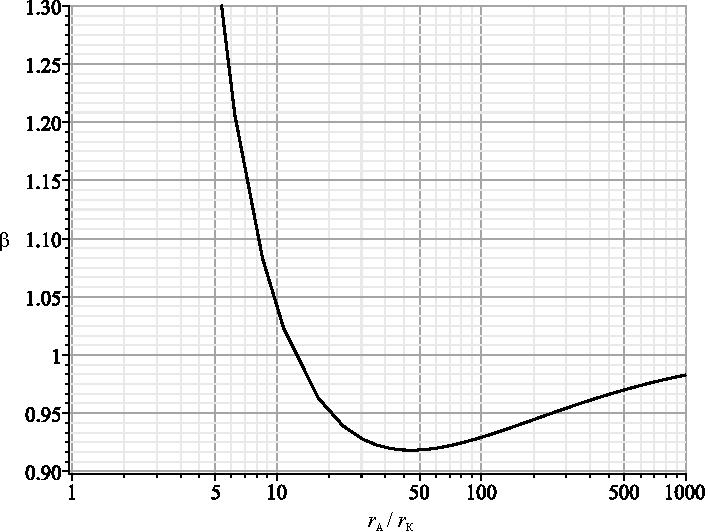
\includegraphics[scale=0.9]{beta.pdf}\par
    \caption{Зависимость поправочного коэффициента $\beta$ от отношения радиусов
        электродов}
    \figmark{beta}
\end{figure}


\experiment 

Исследования проводятся на диоде с косвенным накалом (ток пропускается через 
расположенную вблизи катода \emph{нить накала}). Радиус его 
катода~$r_{К}$, анода~$r_{А}$, а также длина его активной области~$l$ 
указаны на установке. Отметим, что длина
активной области диода (участка катода, покрытого оксидным слоем, обеспечивающим
термоэмиссию электронов) обычно существенно меньше полной
высоты анода (примерно в два раза). Благодаря этому рабочая часть катода достаточно 
удалена от его торцов, и следовательно,
электрическое поле в активной части диода с хорошей точностью можно считать радиальным.

Схема экспериментальной установки изображена на рис.~\figref{Scheme}. Для
питания цепи накала и анода используются два регулируемых источника напряжения. 
Ток накала $I_{н}$ измеряется амперметром, включённым последовательно с
балластным сопротивлением $R$. Анодное напряжение~$U$ измеряется вольтметром, 
а анодный ток $I$~--- миллиамперметром.
В~работе предлагается измерять анодные токи и напряжения в широком диапазоне 
значений (перекрывающем примерно три порядка величины), 
поэтому вольтметр и миллиамперметр должны быть оснащены устройствами 
ручного или автоматического переключения диапазонов измерения.

\begin{figure}[h!]
    \centering
    \pic{9cm}{Chapter_3/3_2_2}
    \caption{Схема экспериментальной установки}
    \figmark{Scheme}
\end{figure}

\labtask

В~работе предлагается исследовать вольт-амперные характеристики диода при
различных токах накала и по результатам
измерений определить удельный заряд электрона.

\begin{lab:task}
    
\item Настройте измерительные приборы согласно прилагаемой к установке
инструкции.

\item Перед включением питания установите ручки регулировки источников
в минимальное положение.

\item Установите минимальный ток накала диода~$I_\text{н}$, 
и минимальное значение анодного напряжения~$V_{A}$, 
указанные в инструкции. Дайте лампе прогреться в течение 5--10 минут.

\item Проведите подробные измерения вольт-амперных характеристик диода 
$I(U)$ во всём допустимом диапазоне изменения напряжений  (см. инструкцию
к установке). 

Всего должно быть измерено не менее 25--30 точек, 
не менее чем по 8--10 на каждый диапазон изменения напряжений. 
Как правило, рекомендуется провести и измерения в диапазоне от 0,5 до 50~В, 
при этом для малых напряжений (до 5~В) измерения рекомендуется производить 
с шагом 0,5~В, для средних (до 15~В)~--- с шагом 1~В и 
для более высоких~--- с шагом 5~В.

\item Повторите измерения вольт-амперных характеристик 
еще при 2--3 рекомендованных значениях токах накала.

\tasksection{Обработка результатов}

\item По результатам проведенных измерений постройте 
вольт-амперные характеристики диода 
в двойном логарифмическом масштабе
$\log I (\log U)$
для каждого тока накала. По графикам определите участки, на которых
выполняется <<закон 3/2>>.

\item Используя данные, соответствующие участкам применимости
<<закона 3/2>>, постройте для каждого тока накала вольт-амперные 
характеристики в координатах $I(U^{3/2})$. 
Убедитесь в том, что зависимость имеет линейный характер. 

\item Найдите наклоны прямолинейных участков зависимости
$I(U^{3/2})$. Используя формулы \eqref{UI_inf}, \eqref{3.2.8}, 
определите удельный заряд электрона~$e/m$.

\item Оцените погрешность результата и сравните его с табличным.

\end{lab:task}


\begin{lab:questions}
    
    \item Каковы условия применимости <<закона 3/2>> для вакуумного диода?
    Почему закон неприменим при малых и больших напряжениях?
    
    \item Изобразите качественно зависимость тока диода от напряжения
    во всём диапазоне положительных напряжений $U_{А}>0$ на аноде.
    
	\item Нарисуйте качественные графики распределения потенциала $\varphi(r)$ 
    между катодом и анодом: а)~в режиме объёмного заряда;
б)~в режиме насыщения тока диода. Объясните эти зависимости.

    \item Как выглядит вольт-амперная характеристика диода при отрицательных
    напряжениях на аноде, $U_{А}<0$?

	\item Как влияет ток накала катода на ток диода при неизменном напряжении
на аноде? Приводит ли это к погрешности измерения~$e/m$?

    \item Получите уравнение \eqref{3.2.1} из интегральной формы теоремы Гаусса
    для электрического поля.
    
    \item Оцените, при каком токе через диод нельзя пренебрегать
    действием магнитного поля этого тока на движение электронов.

\end{lab:questions}

\begin{lab:literature}
	\item \SivuhinIII~--- \S\S100--102.
	\item \Kalashnikov~--- \S157.
\end{lab:literature}


\newpage
\lab{Опыт Милликена.}

\aim{измерение элементарного заряда методом масляных капель.}

\equip{плоский конденсатор в защитном кожухе, осветитель, измерительный микроскоп, электростатический вольтметр,
электронный секундомер, переключатель напряжения, пульверизатор с маслом.}


Идея опыта очень проста. Если элементарный заряд действительно существует, то заряд $q$ любого тела может принимать
только дискретную последовательность значений:
\begin{equation}
	q=0,\,\pm e,\,\pm 2e,\,\pm 3e,\,\ldots\pm ne,\,\ldots,
	\eqmark{3.3.1}
\end{equation}
где $e$~--- элементарный заряд. В предлагаемом опыте измеряется заряд небольших капелек масла, несущих всего несколько элементарных зарядов. Сравнивая между собой заряды капель, можно убедиться, что все они по модулю кратны одному и тому же числу, которое равно, очевидно, элементарному заряду.

Для измерения заряда капель будем исследовать их движение в вертикальном электрическом поле.

Движение заряженной капли в электрическом поле зависит как от электрических сил, так и от массы капли. Масса капли может быть определена по скорости её падения в отсутствие поля.

Рассмотрим свободное падение капли. Уравнение её движения при падении имеет вид
\begin{equation}
	m\frac{dv}{dt}=mg-F_\text{тр},
	\eqmark{3.3.2}
\end{equation}
где $m$~--- масса капли, $v$ --- её скорость, $g$~--- ускорение свободного падения, а $F_\text{тр}$~--- сила вязкого трения капли в воздухе, которая для сферической капли определяется формулой Стокса:
\begin{equation}
	F_\text{тр}=6\pi\eta rv=kv.
	\eqmark{3.3.3}
\end{equation}

Здесь $r$~--- радиус капли, $\eta$~--- коэффициент вязкости воздуха, $k=6\pi\eta r$. Подставляя \eqref{3.3.3} в \eqref{3.3.2}, получим
\begin{equation}
	m\frac{dv}{dt}=mg -kv.
	\eqmark{3.3.4}
\end{equation}

Можно убедиться, что при нулевой начальной скорости решение этого уравнения имеет вид
\begin{equation}
	v=\frac{mg }{k}\left(1-e^{-kt/m}\right).
	\eqmark{3.3.5}
\end{equation}

Установившееся значение скорости равно
\begin{equation}
	v_\text{уст}=\frac{mg }{k}=\frac{\frac 43 \pi\rho r^3g }{6\pi\eta r}=\frac29\frac{\rho}{\eta}g r^2,
	\eqmark{3.3.6}
\end{equation}
где $\rho$~--- плотность масла. Заметим, что \eqref{3.3.6} может быть немедленно получено из \eqref{3.3.4}, если положить $dv/dt=0$.

Как следует из \eqref{3.3.5}, установление скорости происходит с постоянной времени
\begin{equation}
	\tau=\frac{m}{k}=\frac 29 \frac{\rho}{\eta}r^2.
	\eqmark{3.3.7}
\end{equation}
Время установления скорости, таким образом, быстро падает с уменьшением радиуса капли $r$. Для мелких капель оно столь мало, что движение капли всегда можно считать равномерным. Выражение \eqref{3.3.6} в этом случае позволяет определить радиус капли, зная скорость её падения. Обозначая через $h$ путь, пройденный каплей за время $t_0$, найдём
\begin{equation}
	r=\sqrt{\frac{9\eta h}{2\rho g t_0}}.
	\eqmark{3.3.8}
\end{equation}

Рассмотрим теперь движение капли при наличии электрического поля плоского конденсатора, пластины которого расположены горизонтально. Напряжённость поля $E$ в конденсаторе равна
\begin{equation}
	E=\frac{V}{l},
	\eqmark{3.3.9}
\end{equation}
где $l$~--- расстояние между пластинами, а $V$~--- разность потенциалов между ними.

Нас будет интересовать случай, когда под действием электрического поля капля поднимается. Уравнение движения при этом примет вид
\begin{equation}
	m\frac{dv}{dt}=\frac{qV}{l}-mg -kv,
	\eqmark{3.3.10}
\end{equation}
где $q$~--- заряд капли. Появление в правой части постоянного слагаемого не изменяет постоянной времени $\tau$. Для
определения установившейся скорости мы можем снова положить левую часть \eqref{3.3.10} равной нулю.

Измерим время $t$ подъёма капли на начальную высоту. Используя равенства \eqref{3.3.4}, \eqref{3.3.8} и \eqref{3.3.10}, найдём, что заряд капли равен
\begin{equation}
	q=9\pi\sqrt{\frac{2\eta^3 h^3}{g \rho}}\cdot\frac{l(t_0+t)}{Vt_0^{3/2} t}.
	\eqmark{3.3.11}
\end{equation}

Вывод формулы \eqref{3.3.11} предоставляем читателю.

\experiment Схема установки представлена на рис.~\figref{fig3.3.1}. Масло разбрызгивается пульверизатором. Капли масла попадают в конденсатор $C$ через небольшое отверстие в верхней пластине. При этом часть из них вследствие трения о воздух приобретает случайный по абсолютной величине и знаку электрический заряд.

Напряжение на пластины подаётся с регулируемого выпрямителя и измеряется вольтметром $V$. Ключ $K$ позволяет менять направление поля в конденсаторе, чтобы можно было работать  как с отрицательно, так и с положительно заряженными каплями. При размыкании ключа $K$ конденсатор разряжается через дополнительное сопротивление $R\approx 10$~МОм.
\begin{figure}[h!]
	\pic{0.9\textwidth}{3_3_1}
	\caption{Схема экспериментальной установки для измерения заряда электрона}
	\figmark{fig3.3.1}
\end{figure}
Время отсчитывается по электронному секундомеру.

Естественно, что слабые электрические силы, действующие на каплю, несущую всего один или несколько электронных зарядов, способны существенно изменить её движение только в том случае, если сама она очень мала. Опыт производится поэтому с мелкими каплями, наблюдение за которыми возможно только с помощью микроскопа.

В фокальной плоскости окуляра измерительного микроскопа $M$ виден ряд горизонтальных линий, расстояние между которыми было предварительно определено с помощью объектного микрометра. Для облегчения процесса измерений микроскоп может снабжаться камерой с выводом изображения на дисплей ПК. Наблюдая за перемещением капли между линиями, нетрудно определить путь, пройденный каплей. Время $t_0$ свободного падения капли от одной выбранной линии до другой и время $t$ её обратного подъёма, происходящего под действием сил электрического поля, измеряется электронным секундомером.

Из постановки опыта очевидно, что дискретность заряда может быть обнаружена лишь в том случае, если ошибка $\delta q$ в измерении заряда капли существенно меньше абсолютной величины заряда электрона $e$. Допустимая относительная ошибка опыта $\delta q/q$ должна быть поэтому много меньше $e/q=1/n$, где $n$~--- заряд капли, выраженный в числе зарядов электрона. Этому условию тем легче удовлетворить, чем меньше число $n$. В нашем случае трудно определить $q$ с точностью лучше 5\%. Заряд капли должен поэтому быть существенно меньше 20 зарядов электрона~--- лучше всего, если он не превосходит пяти электронных зарядов.

Из всех величин, входящих в формулу \eqref{3.3.11}, на опыте измеряются только $t_0$, $t$, и $V$. От точности определения этих величин зависит в основном ошибка измерения $q$. Из формулы \eqref{3.3.11} можно найти
\begin{equation}
	\frac{\sigma_q}{q}=\sqrt{\frac{\sigma^2_V}{V^2}+\frac{\sigma^2_t t_0^2}{t^2(t_0+t)^2}+
	\frac{\sigma^2_{t_0}}{4t^2_0}\left(\frac{3t+t_0} {t+t_0}\right)^2}.
	\eqmark{3.3.12}
\end{equation}

При $t\approx t_0$ эта формула приобретает вид
\begin{equation}
	\frac{\sigma_q}{q}=\sqrt{\frac{\sigma^2_V}{V^2}+ \frac{\sigma^2_t}{4t^2_0}+ \frac{\sigma^2_{t_0}}{t^2_0}}.
	\eqmark{3.3.13}
\end{equation}

В условиях нашей работы наибольшее влияние на точность эксперимента оказывают два последних стоящих под корнем члена. Ошибка измерения времени $t_0$ и $t$ при визуальном наблюдении капель не может быть сделана меньше 0,1 -- 0,2 секунды. Погрешность в измерении $q$ будет поэтому тем меньше, чем большие значения принимают $t_0$ и $t$. Для увеличения $t_0$ и $t$ можно было бы увеличить расстояние, проходимое каплями, но это сильно усложнило бы экспериментальную установку. Удобнее идти в другом направлении~--- работать с медленно движущимися каплями, т.е. с каплями малого веса. Время падения $t_0$ таких капель достаточно велико. Чтобы время подъёма $t$ было также достаточно большим, нужно использовать не очень большие разности потенциалов $V$.

Заметим, что выбор слишком маленьких капель приводит к снижению точности измерений. Броуновское движение малых капель оказывает существенное влияние на их движение и способно заметно исказить картину их падения и подъёма. Маленькие капли могут испаряться, так что их размеры во время наблюдения могут уменьшаться. При малых скоростях движения делаются особенно опасными конвекционные потоки воздуха, которые возникают при неоднородном нагреве установки (происходящем, например, от осветителя камеры). Практически в наших условиях удобно выбирать $t_0\approx t\approx 10$ -- 30 секунд.

Для капель очень малого размера формула Стокса не вполне применима. Использование формулы Стокса без поправок, впрочем, в наших условиях приводит к искажению значений $q$ и $e$ не более чем на 10\% и почти не мешает обнаружению дискретности электрического заряда. Мы рекомендуем поэтому не вводить в формулу никаких поправок.

\begin{lab:task}

В работе предлагается по измерениям времени свободного падения заряженных капель и времени их подъёма в электрическом поле определить заряд электрона.

\begin{enumerate}

\item{Перед началом работы оцените с помощью формулы \eqref{3.3.11} величину напряжения $V$, которое нужно для подъёма капель, несущих от 1 до 5 зарядов электрона на высоту $h=1$~мм, задав $t_0\approx t=20$~с. Если для подъёма капель потребуются меньшие напряжения, то соответствующие капли слишком сильно заряжены и для эксперимента непригодны.

При вычислениях потребуются значения некоторых величин: расстояние между пластинами $l=0,725$~см; плотность масла
$\rho=0,898$~г/см$^3$; коэффициент внутреннего трения воздуха $\eta=1,83\cdot 10^{-4}$~Пуаз~(СГС) или $1,83\cdot 10^{-5}$~Па$\cdot$с (СИ).}

\item{Включите осветитель. При этом падающий в камеру свет направлен под углом к оси микроскопа и в объектив не попадает. Поле зрения микроскопа остаётся поэтому тёмным. Капли масла рассеивают свет и кажутся светящимися точками на темном фоне.

Не включая электрическое поле \important{слегка} надавите на грушу пульверизатора  и наблюдайте за движением облачка масляных капель в поле зрения микроскопа (изображение перевёрнуто).}

\item{Настройте окуляр микроскопа на резкое изображение делений окулярной шкалы. Затем сфокусируйте объектив на появившиеся в рабочем пространстве капли.}

\item{Наблюдая за движением капель, следует выбирать капли, время падения которых на $h=1$~мм лежит в пределах
10 -- 30 секунд, и научиться отличать их от более крупных, непригодных для работы. Цена деления окулярной шкалы указана на установке.

В случае отсутствия в составе установки ПК с камерой регулировкой и коммутацией напряжения занята одна рука наблюдателя. Вторая рука управляет секундомером. Запись результатов измерений ($t_0$, $t$ и $V$) ведёт второй экспериментатор. Наблюдатель быстро устаёт, поэтому рекомендуется периодически меняться местами. В случае наличия ПК указанные трудности отсутствуют, и работа может быть выполнена одним экспериментатором.

Для уменьшения ошибок в определении $t_0$ и $t$ нужно для пуска и остановки секундомера использовать один и тот же признак~--- всегда нажимать головку секундомера либо в тот момент, когда капля скрывается за линией шкалы, либо, наоборот, когда она появляется из-за линии. Рекомендуется следить за каплей, не отрываясь от окуляра микроскопа, так как в противном случае легко её потерять из виду и весь эксперимент придётся повторить.}

\item{В начале опыта следует позволить капелькам свободно падать \mbox{5 -- 10}~секунд при выключенном электрическом поле для того, чтобы наиболее крупные капли успели упасть на нижнюю пластину.

Из оставшихся в поле зрения капель выберите одну и произведите с ней серию измерений, наблюдая её падение под действием силы тяжести и подъём под действием электрического поля. Серия должна состоять из 5 -- 10 измерений $t_0$ и такого же числа измерений $t$ для одной капли.}

\item{Необходимо проделать не менее 15 таких серий измерений (для 15~различных капель), каждый раз регистрируя величину $V$. При этом нужно иметь в виду, что заряд капли может измениться во время наблюдений; в последнем случае для одной капли получится несколько значений $q$.

Изменение заряда капли может произойти при её подъёме в электрическом поле. Вычисленное с помощью \eqref{3.3.11} значение заряда будет в этом случае соответствовать некоторому среднему из величины заряда капли в начале и в конце опыта. Соответствующий результат непригоден для обработки и только запутывает опыт. Нужно поэтому стараться вовремя отбросить все случаи, когда перезарядка капли произошла во время её подъёма. Это можно сделать, внимательно наблюдая за движением капли и отбрасывая опыты, в которых капля изменила скорость подъёма во время измерения.}

\item{Для оценки точности измерений <<подвесьте>> одну из капель в электрическом поле. Определите соответствующее напряжение, отключите его  и измерьте время падения капли на расстояние 2 -- 3-х делений шкалы. Поменяв полярность напряжения, верните каплю на прежнее место и снова подвесьте её. Снова запишите напряжение. Повторите  процедуру  для одной капли несколько раз  и на месте оцените из этого опыта заряд капли по формуле \eqref{3.3.11}, полагая время подъёма $t=\infty$. По разбросу результатов ($\Delta V$ и  $\Delta t$) оцените точность измерения заряда этой капли.}

\end{enumerate}

\tasksection{Обработка результатов}

\begin{enumerate}

\item{Для всех исследованных капель рассчитайте значения $q$, отложите их на горизонтальной числовой оси и найдите для них общий наибольший делитель. Этот наибольший делитель, вообще говоря, может оказаться равным $e$, $2e$, $3e$ и т.~д. Однако, чем больше значений $q$ было измерено на опыте, тем меньше вероятность получить в качестве делителя число, отличное от $e$. Найденное значение $e$ приведите в системе единиц СИ и в системе СГС.}

\item{Оцените время релаксации $\tau=v_\text{уст}/g$ и расстояние $s$, которое прошла бы капля за это время с установившейся скоростью:
\begin{equation*}
	s=v_\text{уст}\tau=\frac{1}{g}\left(\frac{h}{t_0}\right)^2.
\end{equation*}}

\end{enumerate}

\end{lab:task}

\begin{lab:questions}

\item{Почему не следует выбирать капли слишком большого и слишком маленького размера?}

\item{Какие напряжения соответствуют оптимальным условиям опыта? Приведите расчёты.}

\item{Нарисуйте график зависимости скорости капли в поле силы тяжести от времени и укажите на нём время и путь релаксации.}

\item{Зная параметры установки, оцените ёмкость конденсатора~$C$ и время его разрядки через сопротивление~$R$ (площадь пластин ${\approx} 20$~см$^2$).}

\item{$^*$ Какие ещё способы измерения заряда электрона вам известны?}

\end{lab:questions}

\begin{lab:literature}

\item{ \emph{Сивухин Д.В.} Общий курс физики. Т.~III. Электричество. --- М.:Физматлит, 2015. Гл.~V, \S~90.}

\item{ \emph{Калашников С.Г.} Электричество.~--- М.: Физматлит, 2003. Гл.~XVII, \S~178.}

\end{lab:literature}
\lab{Эффект Холла в полупроводниках}

\aim{измерение подвижности и концентрации носителей заряда в полупроводниках.}

\equip{электромагнит с источником питания, амперметр, миллиамперметр, милливеберметр, реостат, цифровой вольтметр,
источник питания (1,5~В), образцы легированного германия.}

Элементарная теория свободных носителей заряда в~металлах и полупроводниках изложена во введении к разделу.

{\bf Экспериме
нтальная установка.} Электрическая схема установки для измерения ЭДС~Холла представлена на рис.~\ref{fig3.4.1}.

В~зазоре электромагнита (рис.~\ref{fig3.4.1}а) создаётся постоянное магнитное поле, величину которого можно менять с~помощью регулятора~$R_1$ источника питания электромагнита. Ток питания электромагнита измеряется амперметром~А$_1$. Разъём~К$_1$ позволяет менять направление тока в~обмотках электромагнита.

Градуировка магнита проводится при помощи милливеберметра. Описание милливеберметра и правила работы с ним приведены на с.~\pageref{MWB}.

\begin{figure}
%\fcpic[0.9]{3_4_1}
\caption{Схема установки для исследования эффекта Холла в~полупроводниках}
\label{fig3.4.1}
\end{figure}

Образец из легированного германия, смонтированный в~специальном держателе (рис. \ref{fig3.4.1}б), подключается к~источнику питания ($\simeq 1,5$~В). При замыкании ключа~К$_2$ вдоль длинной стороны образца течёт ток, величина которого регулируется реостатом~$R_2$ и измеряется миллиамперметром~А$_2$.

В образце с током, помещённом в зазор электромагнита, между контактами 3 и 4 возникает разность потенциалов~$U_{34}$, которая измеряется с~помощью цифрового вольтметра.

Иногда контакты 3 и 4 вследствие неточности подпайки не лежат на одной эквипотенциали, и тогда напряжение между ними связано не только с~эффектом Холла, но и с~омическим падением напряжения, вызванным протеканием основного тока  через образец. Измеряемая разность потенциалов при одном направлении магнитного поля равна сумме ЭДС~Холла и омического падения напряжения, а при другом~--- их разности. В~этом случае ЭДС ~Холла~$\epsilon_x$ может быть определена как половина алгебраической разности показаний вольтметра, полученных для двух противоположных направлений магнитного поля в~зазоре. Знак измеряемого напряжения высвечивается на цифровом табло вольтметра.

Можно исключить влияние омического падения напряжения иначе, если при каждом токе через образец измерять напряжение
между точками 3 и 4 в~отсутствие магнитного поля. При фиксированном токе через образец это дополнительное к~ЭДС~Холла напряжение~$U_0$ остаётся неизменным. От него следует (с~учётом знака) отсчитывать величину ЭДС~Холла:
\begin{equation}
\epsilon_x=U_{34}\pm U_0.
\label{fig3.4.1}
\end{equation}
При таком способе измерения нет необходимости проводить повторные измерения с~противоположным направлением магнитного поля.

По знаку $\epsilon_x$ можно определить характер проводимости~--- электронный или дырочный. Для этого необходимо знать
направление тока в~образце и направление магнитного поля.

Измерив ток~$I$ в об
разце и напряжение~$U_{35}$ между контактами~3 и 5 в~отсутствие магнитного поля, можно, зная
параметры образца, рассчитать проводимость материала образца по формуле
\begin{equation}
\sigma=\frac{I\, L_{35}}{U_{35}\,a\,l},
\label{eq3.4.2}
\end{equation}
где $L_{35}$~--- расстояние между контактами 3 и 5, $a$~--- толщина образца, $l$~--- его ширина.

{\Large \bf ЗАДАНИЕ}

В работе предлагается исследовать зависимость ЭДС~Холла от величины магнитного поля при различных токах через образец для определения константы Холла; определить знак носителей заряда и проводимость материала образца.

\begin{enumerate}
\item{ Подготовьте приборы к работе.}

\item{ Проверьте работу цепи питания образца. Ток через образец не должен превышать 1~мА.}

\item{ Проверьте работу цепи магнита. Определите диапазон изменения тока через магнит.}

\item{ Прокалибруйте электромагнит~--- определите связь между индукцией~$B$ магнитного поля в зазоре электромагнита и током $I_M$ через обмотки магнита. Для этого с помощью милливеберметра снимите зависимость магнитного потока $\Phi$, пронизывающего пробную катушку, находящуюся в~зазоре, от тока~$I_M$ ($\Phi=BSN$). Значение $SN$ (произведение площади сечения контура катушки на число витков в ней) указано на держателе катушки.}

\item{ Проведите измерение ЭДС Холла. Для этого вставьте образец в~зазор выключенного электромагнита и определите напряжение~$U_0$ между холловскими контактами 3 и 4 при минимальном токе через образец ($\simeq 0,2$~мА). Это напряжение~$U_0$ вызвано несовершенством контактов~3, 4 и при фиксированном токе через образец остаётся неизменным. Значение~$U_0$ с~учётом знака следует принять за нулевое.

Включите электромагнит и снимите зависимость напряжения~$U_{34}$ от тока~$I_M$ через обмотки магнита при фиксированном токе через образец.

Проведите измерения $U_{34}=f(I_{M})$ при постоянном токе через образец для 6--8 его значений в~интервале 0,2--1~мА. При каждом новом значении тока через образец величина~$U_0$ будет иметь своё значение.

При максимальном токе через образец ($\simeq 1$~мА) проведите измерения $U=f(I_{M})$ при другом направлении магнитного поля.
}
\item{ Определите знак носителей в образце. Для этого необходимо знать направление тока через образец, направление магнитного поля и знак ЭДС Холла.

Направление тока в образце показано знаками~<<+>> и <<$-$>> на рис. \ref{fig3.4.1}. Направление тока в~обмотках электромагнита при установке разъёма~K$_1$ в~положение~I показано стрелкой на торце магнита.

Зарисуйте в тетради образец. Укажите на рисунке направления тока, магнитного поля и отклонение носителей. По знаку
($\pm$) на клеммах цифрового вольтметра определите характер проводимости.
}
\item{Для определение удельной проводимости удалите держатель с~образцом из зазора. Подключите к~клеммам~<<$H_{x}$>> и <<$L_{x}$>> вольтметра потенциальные концы~3 и 5. Измерьте падение напряжения между ними при токе через образец 1~мА.}

\item{ Запишите характеристики приборов и параметры образца $L_{35}$, $a$, $l$, указанные на держателе.}
\end{enumerate}

{\rm Обработка результатов}
\begin{enumerate}

\item {Постройте график зависимости $B=f(I_{M})$.}

\item{ Рассчитайте ЭДС~Холла по формуле~(\ref{eq3.4.1}) и постройте на одном листе семейство характеристик $\epsilon_x=f(B)$ при разных значениях тока~$I$ через образец. Определите угловые коэффициенты~$k(I)=\Delta{\epsilon_x}/\Delta B$ полученных прямых.

Постройте график $k=f(I)$. Рассчитайте угловой коэффициент прямой и по формуле~(TO ADD REF) Приложения определите величину постоянной Холла~$R_{X}$. Рассчитайте концентрацию~$n$ носителей тока в~образце по формуле ([TO ADD REF]).

Оцените погрешность результата и сравните результат с~табличным.}


\item{ Рассчитайте удельную проводимость~$\sigma$ материала образца по формуле~(\ref{eq3.4.2}).

Используя найденные значения концентрации~$n$ и проводимости~$\sigma$, с~помощью формулы~([TO ADD REF]) вычислите подвижность~$b$ носителей тока в~общепринятых для этой величины внесистемных единицах: размерность напряжённости электрического поля $[E]=[U/L]=$~B/см, размерность скорости $[v]=$~см/с, поэтому размерность
подвижности~$[b]=$см$^2$/(В$\cdot$с).

Оцените погрешности и сравните результаты с~табличными.}
\end{enumerate}

{\small

{\bf \Large Контрольные вопросы}
\begin{enumerate}



\item{ Какие вещества называют диэлектриками, проводниками, полупроводниками? Чем объясняется различие их электрических свойств? Как зависит от температуры проводимость металлов и полупроводников?}

\item{ Дайте определение константы Холла. Как зависит константа Холла от температуры у металлов и полупроводников?}

\item{ Зависит ли результат измерения константы Холла от геометрии образца?}

\item{ Как устроен милливеберметр? Зависят ли его показания от сопротивления измерительной катушки? Каким должно быть это сопротивление по сравнению с сопротивлением катушки прибора: большим или маленьким?}

\item{ Получите выражение константы Холла для материалов с~двумя типами носителей. При выводе используйте условие равенства нулю поперечного тока.}

\end{enumerate}

{\bf \Large Список литераратуры}

\begin{enumerate}


\item{ \emph{Сивухин Д.В.} Общий курс физики. Т.~III. Электричество~--- М.: Наука, 1983. \S\S~98, 100.}

\item{ \emph{Парселл Э.} Электричество и магнетизм.~--- М.: Наука, 1983. Гл.~4, \S\S~4--6; Гл.~6, \S~9 (Берклеевский курс физики. Т.~II).
    }

\end{enumerate}
}



{\large \bf 3.3.5 Эффект Холла в металлах}

{\bf Цель работы:}{измерение подвижности и концентрации носителей заряда в металлах.}

{\bf В работе используются:}{электромагнит с источником питания, источник постоянного тока, микровольтметр Ф116/1, амперметры, милливеберметр,
образцы из меди, серебра и цинка.}

Элементарная теория свободных носителей заряда в~металлах и полупроводниках изложена во введении к разделу.

{\bf Экспериментальная установка.} Электрическая схема установки для измерения ЭДС~Холла представлена на рис.~\ref{fig3.5.1}.

\begin{figure}
%\fcpic[0.9]{3_5_1}
\caption{Схема установки для исследования эффекта Холла в~металлах}
\label{fig3.5.1}
\end{figure}

В зазоре электромагнита (рис \ref{fig3.5.1}а) создаётся постоянное магнитное поле, величину которого можно менять с~помощью источника питания электромагнита. Разъём~К$_1$ позволяет менять направление тока в~обмотках электромагнита. Ток питания электромагнита измеряется амперметром~А$_1$.

Градуировка магнита проводится с~помощью милливеберметра. Описание милливеберметра и правила работы с ним приведены на с.~\pageref{MWB}.

Металлические образцы в форме тонких пластинок, смонтированные в~специальных держателях, подключаются к~блоку питания через разъём (рис \ref{fig3.5.1}б). Ток через образец регулируется реостатом~$R_2$ и измеряется амперметром~А$_2$.

Для измерений ЭДС Холла используется микровольтметр Ф116/1, в~котором высокая чувствительность по напряжению сочетается с~малой величиной тока, потребляемого измерительной схемой: минимальный предел измерения напряжения составляет~1,5~мкВ, а потребляемый ток~--- всего~$10^{-8}$~А.

В~образце с~током, помещённом в~зазор электромагнита, между контактами~2 и 4 возникает холловская разность потенциалов, которая измеряется с~помощью микровольтметра, если переключатель К$_3$ подключён к~точке~2 образца. При подключении К$_3$ к~точке~3 микровольтметр измеряет омическое падение напряжения~$U_{34}$, вызванное основным током через образец. При нейтральном положении ключа входная цепь микровольтметра разомкнута.

Ключ К$_2$ позволяет менять полярность напряжения, поступающего на вход микровольтметра.

Иногда контакты~2 и 4 вследствие неточности подпайки не лежат на одной эквипотенциали, и тогда напряжение между ними связано не только с~эффектом Холла, но и с~омическим падением напряжения, вызванным протеканием основного тока через образец. Измеряемая разность потенциалов при одном направлении магнитного поля равна сумме ЭДС~Холла и омического падения напряжения, а при другом~--- их разности. В~этом случае ЭДС Холла $\epsilon_x$ может быть определена как половина
алгебраической разности показаний вольтметра, полученных для двух противоположных направлений магнитного поля в~зазоре.


Можно исключить влияние омического падения напряжения иначе, если при каждом токе через образец измерять
напряжение~$U_0$ между точками~2 и 4 в~отсутствие магнитного поля. При фиксированном токе через образец это
дополнительное к ЭДС Холла напряжение остаётся неизменным. От него следует (с~учётом знака) отсчитывать величину
ЭДС Холла:
\begin{equation}
\epsilon_x=U_{24}\pm U_0.
\label{eq3.5.1}
\end{equation}
При таком способе измерения нет необходимости проводить повторные измерения с~противоположным направлением магнитного поля.

По знаку $\epsilon_x$ можно определить характер проводимости~--- электронный или дырочный. Для этого необходимо знать
направление тока в~образце и направление магнитного поля.

Измерив ток $I$ в образце и напряжение~$U_{34}$ между контактами~3 и 4 в~отсутствие магнитного поля, можно, зная
параметры образца, рассчитать проводимость материала образца по очевидной формуле:

\begin{equation}
\sigma=\frac{I\, L_{34}}{U_{34}\, al},
\end{equation}

где $L_{34}$~--- расстояние между контактами~3 и 4, $a$~--- толщина образца, $l$~--- его ширина.

{\Large \bf ЗАДАНИЕ}

В работе предлагается исследовать зависимость ЭДС~Холла от величины магнитного поля при различных токах через образец для определения константы Холла; определить знак носителей заряда и проводимость различных металлических образцов.

\begin{enumerate}

\item{Подготовьте приборы к работе.}

\item{ Проверьте работу цепи питания образца. Для этого подключите к разъёму блока управления один из образцов~--- медный или серебряный. Убедитесь, что ток через образец можно изменять от 0,5 до 1,2~А.}
\item{ Проверьте работу цепи магнита. Установите разъём К$_1$ в положение I и определите диапазон изменения тока через электромагнит.}
\item{ Прокалибруйте электромагнит. Для этого вставьте в зазор электромагнита пробную катушку милливеберметра и исследуйте зависимость магнитного потока~$\Phi$, пронизывающего пробную катушку, от тока $I_M$ через обмотки магнита ($\Phi=BSN$).
Значение $SN$ (площадь сечения пробной катушки на число витков в ней) указано на держателе катушки.

Проведите измерения магнитного потока для 6--8 значений тока через электромагнит.}

\item{ Проведите измерение ЭДС Холла. Для этого вставьте образец в~зазор выключенного электромагнита и определите напряжение~$U_0$ между холловскими контактами 2 и 4 при минимальном токе через образец ($\simeq 0,5$~А). Это напряжение~$U_0$ вызвано несовершенством контактов~2, 4 и при фиксированном токе через образец остаётся неизменным. Значение~$U_0$ с~учётом знака следует принять за нулевое.

Включите электромагнит и снимите зависимость напряжения~$U_{24}$ от тока~$I_M$ через обмотки магнита при фиксированном токе через образец. Измерения следует проводить при {\bf медленном} увеличении магнитного поля. Резкие изменения магнитного поля наводят ЭДС индукции в~подводящих проводах и вызывают большие отклонения стрелки микровольтметра.

Повторите измерения $U=f(I_{M})$ при постоянном токе через образец для 5--6 его значений в~интервале $0,5-1,2$~А. При каждом новом значении тока через образец величина~$U_0$ будет иметь своё значение.

При максимальном токе через образец проведите измерения $U=f(I_{M})$ при другом направлении магнитного поля.

Для образца из цинка снимите зависимость $U=f(I_{M})$ при одном значении тока через образец ($I\simeq 1$~А).}

\item{Определите знак носителей в образце. Для этого необходимо знать направление тока через образец, направление магнитного поля и знак ЭДС Холла. Направление тока в образце показано знаками~<<+>> и <<$-$>> на рис. \ref{fig3.4.1}. Направление тока в~обмотках электромагнита при установке разъёма~K$_1$ в~положение~I показано стрелкой на торце магнита.

Напомним, что знак потенциала, соответствующий точкам 2 или 4, можно определить по рис. \ref{fig3.4.1}.

Зарисуйте в тетради образец. Укажите на рисунке направление тока, магнитного поля (положение разъёма~K$_1$) и знак
потенциала, соответствующий клемме~4 (положение ключа~K$_2$ при отклонении стрелки вольтметра вправо).

Определите знак носителей заряда для каждого из двух образцов.
}
\item{Определите удельную проводимость образца. Для этого удалите держатель с~образцом из зазора. Установите переключатель микровольтметра <<ПРЕДЕЛЫ ИЗМЕРЕНИЯ>> на 750~мкВ. Ключ~K$_3$ поставьте в~положение~$U_{34}$. При токе через образец~$\sim 1$~А измерьте падение напряжения между контактами 3 и 4 для каждого из двух образцов.}

\item{ Запишите характеристики приборов и параметры образцов $L_{34}$ $a$, $l$, указанные на держателях.}
\end{enumerate}

{\rm Обработка результатов}
\begin{enumerate}
\item{Рассчитайте индукцию магнитного поля~$B$ для каждого значения тока и постройте график зависимости $B=f(I_{M})$.}

\item{Рассчитайте ЭДС Холла по формуле~(\r1) и постройте на одном листе семейство характеристик $\epsilon_x=f(B)$ при разных значениях тока~$I$ через образец (для меди или серебра). Определите угловые коэффициенты~$k(I)=\Delta\epsilon/\Delta B$ полученных прямых.}

\item{ Постройте график $k=f(I)$. Рассчитайте угловой коэффициент прямой и по формуле~([TO ADD REF]) определите величину постоянной Холла $R_x$.

Для цинка изобразите на графике зависимость $\epsilon_x=f(B)$ и по наклону прямой рассчитайте постоянную Холла.

Для обоих образцов рассчитайте концентрацию~$n$ носителей тока по формуле ([TO ADD REF]).

Оцените погрешности и сравните результаты с~табличными.}

\item{ Рассчитайте удельную проводимость~$\sigma$ материала образцов по формуле~(\ref{eq3.5.1}).

Используя найденные значения концентрации~$n$ и проводимости~$\sigma$, с~помощью формулы~([TO ADD REF]) рассчитайте подвижность~$b$ носителей тока в~общепринятых для этой величины внесистемных единицах: размерность напряжённости электрического поля~$[E]=[U/L]=В/см$, размерность скорости~$[v]=см/с$, поэтому размерность подвижности $[b]=$см$^2$/(В$\cdot$с).

Оцените погрешности и сравните результаты с табличными.
}
\end{enumerate}

{\small

{\bf \Large Контрольные вопросы}

\begin{enumerate}

\item{ Какие вещества называют диэлектриками, проводниками, полупроводниками? Чем объясняется различие их электрических свойств? Как зависит от температуры проводимость металлов и полупроводников?}

\item{ Дайте определение константы Холла. Как зависит константа Холла от температуры у~металлов и полупроводников?}

\item{ Зависит ли результат измерения константы Холла от геометрии образца?}

\item{ Как устроен милливеберметр? Зависят ли его показания от сопротивления измерительной катушки? Каким должно быть это сопротивление по сравнению с~сопротивлением рамки прибора: большим или маленьким?}

\end{enumerate}

{\bf \Large Список литераратуры}

\begin{enumerate}


\item{ \emph{Сивухин Д.В.} Общий курс физики. Т.~III. Электричество~--- М.: Наука, 1983. \S\S~98, 100.}

\item{ \emph{Парселл Э.} Электричество и магнетизм.~--- М.: Наука, 1983. Гл.~4, \S\S~4--6; Гл.~6, \S~9 (Берклеевский курс физики. Т.~II).}
\end{enumerate}

}



\lab{Влияние магнитного поля на проводимость полупроводников}

\aim{измерение зависимости сопротивления 
    полупроводниковых образцов различной формы от магнитного поля.}

\equip{электромагнит, милливеберметр или миллитесламетр (на основе датчика
Холла), вольтметр, амперметр, миллиамперметр, реостат, образцы
монокристаллического антимонида индия (InSb) $n$-типа.}

Перед выполнением работы необходимо ознакомиться с основами
элементарной теории движения носителей заряда в~металлах и полупроводниках
(п. \ref{sec:halleffect} Введения к разделу).

В работе изучается зависимость проводимости полупроводников от магнитного поля
в геометрии \emph{диска Корбино}.
По диску, помещенному в перпендикулярное ему магнитное поле, пропускается
ток в радиальном направлении. Магнитное поле искривляет линии 
тока, благодаря чему эффективное сопротивление образца возрастает
(эффект \emph{геометрического магнетосопротивления}). По результатам
измерений зависимости сопротивления от магнитного поля 
могут быть вычислены подвижность и концентрация носителей тока в образце.

\experiment
Схема установки для исследования магнетосопротивления
полупроводников и геометрического резистивного эффекта представлена на
рис.~\figref{Scheme}.

\begin{figure}[h!]
    \centering
    \pic{0.9\textwidth}{Chapter_3/3_6_1}
    \caption{Схема установки для~исследования влияния магнитного~поля
        на~проводимость полупроводников}
    \figmark{Scheme}
\end{figure}

В зазоре электромагнита (рис.~\figref{Scheme}а) создаётся постоянное магнитное
поле, величину которого можно менять с помощью источника питания электромагнита.
Ток электромагнита измеряется амперметром А$_1$ (отдельным или встроенным в источник).
Магнитная индукция в зазоре измеряется при помощи милливеберметра (его описание
и правила работы с ним приведены на с.~\pageref{MWB}) или 
миллитесламетра на основе датчика Холла.

Образец в форме кольца (диск Корбино) или пластинки, смонтированный в
специальном держателе, подключается к источнику постоянного напряжения 5~В. При
замыкании ключа~К$_2$ сквозь образец течёт ток, величина которого измеряется
миллиамперметром~А$_2$ и регулируется реостатом~$R_2$. Балластное сопротивление~$R_0$
ограничивает ток через образец. Измеряемое напряжение подаётся на вход
вольтметра~V.

\labtask


В работе предлагается при постоянном токе через образец исследовать зависимость
напряжения на образце от величины магнитного поля и от ориентации образца в
магнитном поле; по результатам измерений рассчитать подвижность электронов,
удельное сопротивление материала образца и концентрацию электронов.

\begin{lab:task}

\item Подготовьте приборы к работе согласно описанию на установке.

\item Концы от точек~3 и~4 разъёма подсоедините к клеммам вольтметра.
Присоедините диск Корбино через разъём к цепи питания. Определите
диапазон изменения силы тока через образец.

\item Установите ручки регулировки источника питания электромагнита 
в минимальное положение и включите источник. 
Плавно меняя ток магнита, определите диапазон его изменения.

\item Измерьте калибровочную кривую электромагнита~---
зависимость между индукцией~$B$ магнитного поля в его зазоре и 
током~$I_{М}$ через обмотки магнита.
Магнитное поле измеряется милливеберметром или миллитесламетром
(датчиком Холла). Калибровочная кривая должна содержать не менее
15 точек во всём диапазоне изменения токов.

В~случае использования милливеберметра измерьте зависимость 
магнитного потока~$\Phi$, пронизывающего пробную катушку, 
находящуюся в зазоре, от тока~$I_{М}$ ($\Phi=BSN$). 
Значение~$SN$ (произведение площади сечения контура катушки на
число витков в ней) указано на держателе катушки.

\item \label{p1} Вставьте образец в зазор \emph{выключенного} электромагнита 
и измерьте падение напряжения $U_0$ в образце при некотором токе,
рекомендованном в описании ($I_0\sim 25$~мА). 

\item \label{p2} Включите электромагнит и измерьте зависимость напряжения~$U$ 
на образце от тока через обмотки магнита~$I_M$ при фиксированном токе
через образец~$I_0$.

\item Проверьте, что результат измерения не зависит от направления магнитного
поля.

%\item Повторите измерения пп. \ref{p1}, \ref{p2} 
%для 3--4 других значений тока $I_0$ через образец.

\item Вместо диска Корбино подключите к измерительной цепи образец, имеющий
форму пластинки. Поместите образец в зазор выключенного электромагнита и
измерьте падение напряжения~$U_0$ на образце при токе через образец $10$~мА.

\item Включите электромагнит и снимите зависимость напряжения~$U$ на образце от
тока через магнит при постоянном токе $I=10$~мА. При измерениях длинная сторона
образца должна быть направлена поперёк поля, а средняя (ширина) в~одной серии
опытов располагается вдоль, а в другой~--- поперёк поля.

\item Запишите геометрические размеры образцов и характеристики приборов.

\tasksection{Обработка результатов}

\item Постройте калибровочный график зависимости $B(I_{M})$. 
    Используйте эту зависимость для дальнейшего пересчёта (интерполяции)
    значений поля по измеренным токам $I_{М}$.

\item Для всех серий измерений постройте графики, отложив по оси абсцисс
величину~$B^2$, а по оси ординат~--- величину $(U-U_0)/U_0$. Какие выводы
можно сделать на основании построенных зависимостей?

\item По наклону прямолинейного участка графика для диска Корбино рассчитайте
с помощью формулы \chaptereqref{MagnetoSoprot} подвижность носителей.

\item Определите сопротивление диска $R_0$ в отсутствие магнитного поля.
По геометрическим размерам образца рассчитайте удельное сопротивление~$\rho_0$ 
и удельную проводимость $\lambda_0=1/\rho_0$ материала образца.

\item С помощью формулы \chaptereqref{3.26} найдите концентрацию носителей
тока.

\item Оцените погрешности и сравните результаты с табличными.

\end{lab:task}


\begin{lab:questions}

\item Какие вещества называют диэлектриками, проводниками, полупроводниками?
Чем объясняется различие их электрических свойств? Как зависит от температуры
проводимость металлов и полупроводников?

\item В чем причина зависимости сопротивления образца от магнитного
поля в геометрии диска Корбино?

\item Зависит ли эффект магнетосопротивления от геометрии образца? 
В каких случаях эффект магнетосопротивления может проявиться
при протекании тока по плоской пластинке?

\item Как устроен милливеберметр? Зависят ли его показания от сопротивления
измерительной катушки? Каким должно быть это сопротивление по сравнению с
сопротивлением рамки прибора: большим или маленьким?

\item По результатам измерений оцените частоту столкновений,
длину пробега и коэффициент диффузии носителей тока в исследуемом материале.

\item Получите выражение для сопротивления пластинки, изготовленной
из материала с~двумя типами носителей. 
Для простоты можно ограничиться случаем $\mu_e \gg \mu_h$.

\end{lab:questions}


\begin{lab:literature}
\item \SivuhinIII~--- \S\S~98, 100.
\item \textit{Парселл Э.} Электричество и магнетизм.~--- М.: Наука, 1983. Гл.~4,
\S\S~4--6; Гл.~6, \S~9.
\end{lab:literature}



\end{document}